\RequirePackage{etoolbox}
\csdef{input@path}{%
	{sty/}% cls, sty files
	{img/}% eps files
}%
\csgdef{bibdir}{bib/}% bst, bib files

\documentclass[ba]{imsart}
%
\pubyear{0000}
\volume{00}
\issue{0}
\doi{0000}
\firstpage{1}
\lastpage{1}

%
\usepackage{amsthm}
\usepackage{amsmath}
\usepackage{natbib}
\usepackage[algo2e]{algorithm2e}
\usepackage{algorithmic}  
\usepackage{algorithm}
\usepackage{mathtools}
\usepackage[colorlinks,citecolor=blue,urlcolor=blue,filecolor=blue,backref=page]{hyperref}
\usepackage{graphicx}
\usepackage{subcaption}

\def\spacingset#1{\renewcommand{\baselinestretch}%
	{#1}\small\normalsize} \spacingset{1}
\usepackage{fmtcount}
\startlocaldefs
\numberwithin{equation}{section}
\theoremstyle{plain}
\newtheorem{thm}{Theorem}[section]
\endlocaldefs
\DeclarePairedDelimiter\abs{\lvert}{\rvert}
\begin{document}
	
	\begin{frontmatter}
		\title{A Network Model for Dynamic Textual Communications
with Application to Government Email Corpora}
		\runtitle{Interaction-Partitioned Topic Model}
		
		\begin{aug}
			\author{\fnms{Bomin} \snm{Kim}\thanksref{addr1,t1,t2,m1}\ead[label=e1]{bzk147@psu.edu}},
			\author{\fnms{Aaron} \snm{Schein}\thanksref{addr2,t3,m1,m2}\ead[label=e2]{aschein@cs.umass.edu}},
			\author{\fnms{Bruce} \snm{A. Desmarais}\thanksref{addr3,t3,m1,m2}\ead[label=e3]{bdesmarais@psu.edu}},
			\and
			\author{\fnms{Hanna} \snm{Wallach}\thanksref{addr4,t1,m2}
				\ead[label=e4]{hanna@dirichlet.net}
				%\ead[label=u1,url]{http://www.foo.com}
			}
			\runauthor{B. Kim et al.}
			
			\address[addr1]{Department of Statistics, Pennsylvania State University
				\printead{e1} % print email address of "e1"
			}
			\address[addr2]{College of Information and Computer Sciences, UMass Amherst
				\printead{e2} % print email address of "e1"
			}
			\address[addr3]{Department of Political Science, Pennsylvania State University
				\printead{e3} % print email address of "e1"
			}
			\address[addr4]{ Microsoft Research NYC
				\printead{e4}
			}
			
			%\thankstext{t1}{Some comment}
			%\thankstext{t2}{First supporter of the project}
			%\thankstext{t3}{Second supporter of the project}
			
		\end{aug}
		
		\begin{abstract}
			We introduce the interaction-partitioned topic
model (IPTM)---a probabilistic model for who
communicates with whom about what, and when.
Broadly speaking, the IPTM partitions timestamped
textual communications, according to
both the network dynamics that they reflect and
their content. To define the IPTM, we integrate the hyperedge event model (HEM)---a generative model for events that can be represented as directed edges with one sender and one or more receivers or one receiver and one or more senders---and
latent Dirichlet allocation (LDA)---a generative model
for topic-based content. The IPTM assigns each
document to an ``interaction pattern"---a generative process for contents and ties that is governed by a topic distribution and a set of dynamic network features. We use the IPTM to analyze emails sent between department managers in Dare county government in North Carolina, and demonstrate that the model is effective at predicting and explaining continuous-time textual communications.		\end{abstract}
		
		\begin{keyword}[class=MSC]
			\kwd[Primary ]{60K35}
			\kwd{60K35}
			\kwd[; secondary ]{60K35}
		\end{keyword}
		
		\begin{keyword}
			\kwd{dynamic network model} 
			\kwd{topic modeling}
			\kwd{text analysis}
			\kwd{email data analysis}
		\end{keyword}
		
	\end{frontmatter}
	
	\section{Introduction}\label{sec:introduction}
In recent decades, real-time digitized textual communication has developed into a ubiquitous form of social and professional interaction \citep{kanungo2008modeling, szostek2011dealing, burgess2004email, pew2016}. From the perspective of the computational social scientist, this has lead to a growing need for methods of modeling interactions that manifest as text exchanged in continuous time. A number of models that build upon topic modeling through Latent Dirichlet Allocation (LDA) \citep{Blei2003} to incorporate link data as well as textual content have been developed recently \citep{mccallum2005author,lim2013twitter,Krafft2012}. These models are innovative in their extensions that incorporate network tie information. However, none of the models that are currently available in the literature integrate the rich random-graph structure offered by state of the art models for network structure---such as the exponential random graph model (ERGM) \citep{robins2007introduction,chatterjee2013estimating,hunter2008ergm}. The ERGM is the canonical model for modeling the structure of a static network. It is flexible enough to specify a generative model that accounts for nearly any pattern of tie formation (e.g., reciprocity, clustering, popularity effects) \citep{desmarais2017statistical}. Several models have been developed that handle time-stamped ties in which tie formation is governed by structural dynamics similar to those used in ERGMs \citep{PerryWolfe2012,Butts2008,snijders1996stochastic}. We develop the interaction-partitioned topic model (IPTM) which simultaneously models the network structural patterns that govern time-stamped tie formation, and the content in the communications.~\looseness=-1

The models on which we build, including the relational event model \citep{Butts2008}, the point process model \citep{PerryWolfe2012}, and most closely the hyperedge event model (HEM), provide frameworks for explaining or predicting ties between nodes using the network sub-structures in which the two nodes are embedded (e.g., predict a tie is highly likely to form between two nodes if those two nodes have many shared partners). Models based on network structure have been used for many applications in which the ties between nodes are annotated with text. The text, despite providing rich information regarding the strength, scope, and character of the ties, has been largely excluded from these analyses, due to the inability of these network models to incorporate textual attributes of ties. These application domains include, among other applicaitons, the study of legislative networks in which networks reflect legislators' co-support of bills, but exclude bill text \citep{bratton2011networks,aleman2013explaining}; the study of alliance networks in which networks reflect countries' co-signing of treaties, but exclude treaty text \citep{camber2010geometry,cranmer2012complex,cranmer2012toward,kinne2016agreeing}; the study of scientific co-authorship networks that exclude the text of the co-authored papers \citep{kronegger2011collaboration,liang2015changing,fahmy2016gender}; and the study of text-based interaction on social media (e.g., users tied via `mentions' on twitter) \citep{yoon2014strategies,peng2016follower,lai2017connecting}.~\looseness=-1

In defining and testing the IPTM we embed core conceptual property---interaction pattern---to link the content component of the model, and network component of the model such that knowing who is communicating with whom at what time (i.e., the network component) provides information about the content of communication, and vice versa (Section \ref{sec:generative process}). The IPTM leads to an efficient inference using the Markov Chain Monte Carlo (MCMC) algorithm (Section \ref{sec:inference}) and acheives good predictive peformance (Section \ref{sec:Emails}). Finally, the IPTM discovers interesting and interpretable latent structure through application to email corpora of internal communications by government officials in Dare County, NC (Section \ref{sec:Emails}). 
~\looseness=-1
	
	\section{Interaction-partitioned Topic Model}\label{sec:generative process}
		In this section we define the IPTM by describing a process according to which documents are generated in continuous time. Data generated under the IPTM consists of $D$ unique documents. A single document indexed by $d \in [D]$---where $[D]$ denotes a categorical set with $D$ levels $[D] = \{1,\ldots,D\}$---is represented by the four components: the sender $s_d \in [A]$, an indicator vector of receivers $\boldsymbol{r}_d$, where $r_{dj}=1$ if $j \in [A]$ is a receiver of document $d$ and 0 otherwise, the timestamp $t_d \in (0, \infty)$, and a set of word counts $\boldsymbol{w}_d= \{w_{dv} \}_{v=1}^{V}$---where each $w_{dv}$ is an integer greater or equal to zero and $V$ is the size of vocabularies---that comprise the text of the document. For simplicity, we assume that documents are ordered by time such that $t_d < t_{d+1}$.~\looseness=-1
		
\subsection{Interaction Patterns}\label{subsec:Interaction patterns}
They key idea that combines the IPTM component modeling ``what" with
the component modeling ``who," ``whom," and ``when" is that different
documents comes from the introduction of ``interaction patterns."  Each interaction pattern $c \in [C]$ is characterized by a set of features that affects networks and timestamps---such as the number of messages sent from $i$ to $j$ in some time interval---and corresponding coefficients. We associate each document with the interaction pattern that best describes how people interact, and that is reflected to what people talk about via topic assignments. To be specific, each document $d \in [D]$ draws an interaction pattern $c_d$
\begin{equation}
c_d\sim \mbox{Categorical}({\psi_1},\ldots,{\psi_C}),
\end{equation}
and we assume the interaction pattern-specific factors are gamma-distributed with $\sum_c \psi_c = 1$ (i.e., Dirichlet distribution) such that 
\begin{equation}
\psi_c\sim \Gamma(\epsilon_0,\epsilon_0),
\end{equation}
where we place an uninformative gamma prior over these shape and rate parameters.~\looseness=-1

\subsection{Generative Process for Network Dynamics}\label{subsec:Tie generating process}	
The generative process for network portion of the documents---the senders, receivers, and timestamps---exactly follows that of the hyperedge event model (HEM), except that now we consider the interaction pattern assignments of the documents in order to understand the differences in network dynamics across the interaction patterns.
While the HEM can be applied for two types of hyperedges---edges with (1) one sender and one or more receivers, and (2) one or more senders and one receiver---here we only present the generative process for those involving one sender and one or more receivers, considering our email applications. %One notable feature of the IPTM generative process is that we draw auxiliary variables that serve as candidate data. Data is generated from the IPTM through a sampling process applied to the auxiliary variables. The auxiliary variables drawn for document $d$ include, for each sender $a$, a time increment from document $d-1$ at which sender $a$ would send document $d$, and an $A-1$ length vector indicating which nodes would receive document $d$ if it were sent by sender $a$.  The data generated for document $d$ under the IPTM corresponds to the sender that would send document $d$ the soonest---at the smallest time increment from document $d-1$. The receivers of document $d$ generated under the IPTM correspond to those receivers to which the sender with the minimum time increment would have sent document $d$. We explain these steps in more detail below. 
~\looseness=-1
\subsubsection{Candidate receivers}\label{subsubsec: Tie}
	Given the interaction pattern of document $d$---i.e., $c_d$, we define the ``receiver intensity" for every possible sender--receiver pair $(i,j)$ where $i \!\neq\! j$ as a linear combination of statistics relevant to the receiver selection process:
	\begin{equation}
		\lambda_{idj} = {\boldsymbol{b}_{c_d}}^{\top}\boldsymbol{x}_{idj{c_d}},
	\end{equation}
	where $\boldsymbol{b}_c$ is a $P$--dimensional vector of coefficients and $\boldsymbol{x}_{idjc}$ is a set of receiver selection features which vary depending on the hypotheses regarding canonical processes relevant to network theory such as popularity, reciprocity, and transitivity, as well as the effects of attributes of the sender and receivers, or sender--receiver pairs. We place a Normal prior $\boldsymbol{b}_c \sim N(\boldsymbol{\mu}_b, \Sigma_b)$.~\looseness=-1
	
	We then draw a binary receiver vector $\boldsymbol{u}_{id}= (u_{id1},
	\ldots, u_{idA})$ from a probability measure ``MB$_{G}$", which helps us to 1) allow a sender to select multiple receivers for a single document, 2) force the sender to select at least one receiver, and 3) ensure a tractable normalizing constant for the receiver selection distribution. To be specific, we assume
	\begin{equation} \boldsymbol{u}_{id}  \sim
		\mbox{MB}_{G}(\boldsymbol{\lambda}_{id}),
	\end{equation}
	where $\boldsymbol{\lambda}_{id}= (\lambda_{id1},\ldots,\lambda_{idA})$. In particular, we define $\mbox{MB}_{G}(\boldsymbol{\lambda}_{id})$ as
	\begin{equation}
		\begin{aligned}
			&\Pr(\boldsymbol{u}_{id}|\boldsymbol{b}, \boldsymbol{x}_{id}, c_d) = \frac{1}{Z(\boldsymbol{\lambda}_{id})}\exp\Big(\mbox{log}\big(\text{I}( \lVert \boldsymbol{u}_{id}\rVert_1 > 0 )\big) + \sum_{j\neq i} \lambda_{idj}u_{idj}\Big) ,
		\end{aligned}
		\label{eqn:Gibbs}
	\end{equation}
	where $Z(\boldsymbol{\lambda}_{id})= \prod_{r \neq a} \big(\mbox{exp}(\lambda_{idj}) + 1\big)-1$ is the normalizing constant and is the $\ell_1$-norm, and the log-indicator term $\mbox{log}\big(\text{I}( \lVert \boldsymbol{u}_{id}\rVert_1 > 0 )\big)$ ensures that empty receiver sets are excluded from the distribution's support. This is approximately equivalent to assuming that each $u_{idj}$ is drawn with the probability of 1 being logit($\lambda_{idj}$), excluding the case when $u_{idj}=0$ for all $j \in [A]$.
	
	\subsubsection{Candidate timestamps}\label{subsubsec:Time}
	Similarly, for each sender and document combination, our model draws a candidate timestamp at which the document would be sent given the candidate sender and receiver combinations. Given the interaction pattern assignment $c_d$, the timing rate for sender $i$ and document $d$ is
	\begin{equation}
		\mu_{id} = g^{-1}(\boldsymbol{\eta}_{c_d}^\top \boldsymbol{y}_{idc_d}),
	\end{equation}
	where $\boldsymbol{\eta}_c$ is a $Q$--dimensional vector of coefficients with a Normal prior $\boldsymbol{\eta}_c \sim N(\boldsymbol{\mu}_\eta,\Sigma_\eta)$, $\boldsymbol{y}_{adc}$ is a set of event timing features---covariates that could affect timestamps of the document, and $g(\cdot)$ is the appropriate link function such as identity, log, or inverse. 
	
	%In modeling ``when," we do not directly model the timestamp $t_d$. Instead, we assume that each sender's ``time increment"---i.e., waiting time to next interaction since $t_{d-1}$---is drawn from a specific distribution in the exponential family. We define the time increment from edge $d-1$ to edge $d$ as $\tau_{d}$ (i.e., $\tau_{d}= t_d-t_{d-1}$) and specify the distribution of candidate timestamps with sender-specfic mean $\mu_{ad}$. 
	Next, following the generalized linear model (GLM) framework \citep{nelder1972generalized}, we assume the mean and variance of the $\tau_{id}$---i.e., each sender's ``time increment" from document $d-1$ to document $d$ or $t_d-t_{d-1}$---satistify
	\begin{equation}
		\begin{aligned}
			E(\tau_{id}) &= \mu_{id},\\
			V(\tau_{id}) &= V(\mu_{id}),
		\end{aligned}
	\end{equation}
	where $\tau_{id}$ here is a positive real number drawn from a specific distribution among the possible choices including exponential, Weibull, gamma, and log-normal. We may need other latent variables to draw the time increment based on the choice of distribution, to account for the variance of time increments, beyond the coefficients for the features used to model the rate. $V(\mu)$---e.g., the shape parameter $k$ for the Weibull, the shape parameter $\theta$ for the gamma, and the variance parameter $\sigma_\tau^2$ for the log-normal. We use $f_\tau(\cdot; \mu, V(\mu))$ and $F_\tau(\cdot; \mu, V(\mu))$ to denote the probability density function (p.d.f) and cumulative density function (c.d.f), respectively, with mean $\mu$ and variance $V(\mu)$.~\looseness=-1
	\subsubsection{Senders, receivers, and timestamps}\label{subsubsec:Observed}
	Finally, under the IPTM the observed sender, receivers, and timestamp of document $d$ is generated by selecting the sender--receiver-set pair with the smallest time increment \citep{snijders1996stochastic}, along with the words generated according to Section \ref{subsec:Content generating process}:
	\begin{equation}
		\begin{aligned}
			s_d &= \mbox{argmin}_{i}(\tau_{id}),\\
			\boldsymbol{r}_d &= \boldsymbol{u}_{s_d d},\\
			t_d &=t_{d-1} + \tau_{s_d d},\\
				%	\boldsymbol{w}_d &=(w_{d1},\ldots,w_{dV})
		\end{aligned}
	\end{equation}
		Therefore, it is a sender-driven process in that the receivers and timestamps of a document are jointly determined by the sender's urgency to send the document to the selected receivers. Note that our generative process accounts for tied events such that in case of tied documents---i.e., multiple senders draw exactly the same candidate timestamps---we assume that all documents are generated and occur simultaneously. 
		\subsection{Generative Process for Contents}\label{subsec:Content generating process}
		
		Given the sender-receiver-timestamps, the words $\boldsymbol{w}_d$ are generated by extending the well-known Bayesian topic model, latent Dirichlet allocation (LDA) \citep{Blei2003}, to follow the form of Bayesian Poisson Tucker decomposition (BPTD) \citep{schein2016bayesian}. As in LDA, we generate the corpus-wide global variables that describe the content via topics. First, the interaction pattern-topic factors for each interaction pattern $c \in [C]$ and the topic-word factors for each topic $k\in [K]$ and word type $v\in [V]$ are both gamma-distributed, where we again assume that these factors are drawn directly from an uninformative gamma prior
		\begin{equation}
			\begin{aligned}
				\theta_{ck}& \sim  \Gamma(\epsilon_0,\epsilon_0),\\
				\phi_{kv}& \sim  \Gamma(\epsilon_0,\epsilon_0).
			\end{aligned}
		\end{equation}
		
		Next, we generate the sender-specific factors for each  $i \in [A]$ from uninformative gamma prior
		\begin{equation}
			\pi_{i}\sim \Gamma(\epsilon_0,\epsilon_0),
		\end{equation}
		which serves as the weight of sender $i$ such that a person with higher weight tends to write a document using more words. Finally, given the specifications above, the number of words of type $v\in [V]$ in document $d$ is drawn from 
		\begin{equation}
			w_{dv} \sim \mbox{Poisson}(\pi_{s_d}\sum_{c=1}^C \sum_{k=1}^K I_{dc} \theta_{ck}\phi_{kv}),
		\end{equation}
		where $I_{dc}$ is an indicator for $I(c_d=c)$. Note that Equation (2.11) above is identical to $w_{dv} \sim \mbox{Poisson}(\pi_{s_d}\sum_{k=1}^K \theta_{c_dk}\phi_{kv})$. Also note that $\boldsymbol{w}_d = (w_{d1},\ldots,w_{dV})$ is a very sparse vector with $\sum(\boldsymbol{w}_d) = N_d$, where $N_d$ denotes the total number of words in a document. Algorithm \ref{alg:generative} provides a summary on Section \ref{sec:generative process}, which presents the entire generative process for documents given the gamma-distributed factors. ~\looseness=-1
	\begin{algorithm}[!t]
		\spacingset{1}
		\SetAlgoLined
		\caption{Generative Process: one sender and one or more receivers}
	\begin{algorithmic}
		\STATE \textbf{Input}: number of documents and nodes $(D, A)$, gamma weights $(\boldsymbol{\psi}, \boldsymbol{\phi},\boldsymbol{\theta},\boldsymbol{\pi})$, covariates $(\boldsymbol{x}, \boldsymbol{y})$, and coefficients $(\boldsymbol{b}, \boldsymbol{\eta})$
		\vskip 0.1in
		\FOR{$d=1$ to $D$}
		\STATE	draw $c_d\sim \mbox{Categorical}({\psi_1},\ldots,{\psi_C})$
			\FOR{$i=1$ to $A$}
		\FOR{$j=1$ to $A$ ($j \neq i$)}
		\STATE	set $\lambda_{idj} = {\boldsymbol{b}^{\top}_{c_d}}\boldsymbol{x}_{idj}$
		\ENDFOR
		\STATE	draw $\boldsymbol{u}_{id}  \sim
		\mbox{MB}_G(\boldsymbol{\lambda}_{id})$
		\STATE		set $\mu_{id} = g^{-1}({\boldsymbol{\eta}^\top_{c_d}} \boldsymbol{y}_{id})$
		\STATE		draw $\tau_{id} \sim f_\tau(\mu_{id}, V(\mu))$
		\FOR{$v=1$ to $V$}
		\STATE $w_{dv} \sim \mbox{Poisson}(\pi_{\mbox{argmin}_{i}(\tau_{id})}\sum_{c=1}^C \sum_{k=1}^K I_{dc} \theta_{ck}\phi_{kv})$
		\ENDFOR
		\ENDFOR
		
		\IF{$n \geq 2$ tied events} 
		\STATE	set $s_d,\ldots, s_{d+n-1}=\mbox{argmin}_{i}(\tau_{id}),$
		\STATE	set $\boldsymbol{r}_d=\boldsymbol{u}_{s_d d},\ldots,\boldsymbol{r}_{d+n-1}=\boldsymbol{u}_{s_{d+n-1} d}$
		\STATE	set $t_d, \ldots, t_{d+n-1}=t_{d-1} + \min_i\tau_{id}$
		\STATE set $\boldsymbol{w}_d=(w_{d1},\ldots,w_{dV})$
		\STATE		jump to $e = d+n$
		\ELSE
		\STATE	set $s_d= \mbox{argmin}_{i}(\tau_{id})$
		\STATE		set $\boldsymbol{r}_d= \boldsymbol{u}_{s_d d}$
		\STATE	set $t_d =t_{d-1} + \min_i\tau_{id}$
			\STATE set $\boldsymbol{w}_d=(w_{d1},\ldots,w_{dV})$
		\ENDIF
		\ENDFOR
	\end{algorithmic}
		\label{alg:generative}
	\end{algorithm}
	\newpage
	\section{Posterior inference}\label{sec:inference}
	In this section we describe how we invert the generative process to obtain the posterior distribution over the latent variables---interaction pattern factors $\{\psi_c\}_{c=1}^C$ and assignments $\{c_d\}_{d=1}^D$, topic-word factors $\{\{\phi_{kv}\}_{v=1}^V\}_{k=1}^K$, interaction pattern-topic factors $\{\{\theta_{ck}\}_{k=1}^K\}_{c=1}^C$, document-specific factors $\{\pi_{i}\}_{i=1}^A$, candidate receivers $\{\boldsymbol{u}_d\}_{d=1}^D$, coefficients for receiver selection features $\{\boldsymbol{b}_c\}_{c=1}^C$, and coefficients for event timing features $\{\boldsymbol{\eta}_c\}_{c=1}^C$---conditioned on the observed data $\{(s_d, \boldsymbol{r}_d, t_d, \boldsymbol{w}_d)\}_{d=1}^D$, covariates $\{(\boldsymbol{x}_d, \boldsymbol{y}_d)\}_{d=1}^D$, and hyperparamters $(\boldsymbol{\mu}_b, \Sigma_b, \boldsymbol{\mu}_\eta, \Sigma_\eta, \gamma_0, \xi, \epsilon_0)$. We draw the samples using Markov chain Monte Carlo (MCMC) methods, repeatedly resampling the value of each latent variable from its conditional posterior via a Metropolis-within-Gibbs sampling algorithm. In the following, we provide each latent variable's conditional posterior along with pseudocode of MCMC in Algorithm \ref{alg:MCMC}.
		\subsubsection{Interaction pattern factors}
		\begin{equation}
		\begin{aligned}
	\Pr(\boldsymbol{\psi}|\boldsymbol{c}) & \propto \Pr(\boldsymbol{c}|\boldsymbol{\psi}) \times \Pr(\boldsymbol{\psi})\\
	& \propto (\prod_{d=1}^D {\psi_{c_d}} )\times \prod_{c=1}^C \psi_c^{\epsilon_0-1}\\
	&\propto\prod_{c=1}^C  (\psi_c)^{\sum_{d=1}^D I_{dc}+\epsilon_0-1}\\
&	\sim Dir(\{\sum_{d=1}^D I_{dc}+\epsilon_0\}_{c=1}^C)
		\end{aligned}	
		\end{equation}
		\subsubsection{Interaction pattern-topic factors}
				\begin{equation}
				\begin{aligned}
				\Pr(\theta_{ck}|\,\boldsymbol{\theta}_{\backslash c,k},\boldsymbol{\phi},\boldsymbol{w},\boldsymbol{\pi},\boldsymbol{c}) & \propto \Pr(\boldsymbol{w}_{ck}|\,\theta_{ck},\boldsymbol{\theta}_{\backslash c,k},\boldsymbol{\phi},\boldsymbol{\pi},\boldsymbol{c}) \times \Pr(\theta_{ck})\\
				& \propto (\prod_{d:c_d=c}\prod_{v=1}^V \frac{(\pi_{s_d} \theta_{ck}\phi_{kv})^{w_{dkv}}\times \exp(-\pi_{s_d} \theta_{ck}\phi_{kv})}{w_{dkv}!} )\times \theta_{ck}^{\epsilon_0-1} \times \exp(-\epsilon_0 \theta_{ck})\\
				&\propto (\theta_{ck})^{\sum_{d:c_d=c}\sum_{v=1}^V w_{dkv}+\epsilon_0-1}\times \exp(-(\epsilon_0 +\sum_{d:c_d=c}\sum_{v=1}^V\pi_{s_d} \phi_{kv})\theta_{ck})\\
				&	\sim \Gamma(\sum_{d:c_d=c}\sum_{v=1}^V w_{dkv}+\epsilon_0, \sum_{d:c_d=c}\sum_{v=1}^V\pi_{s_d} \phi_{kv}+\epsilon_0),
				\end{aligned}	
				\end{equation}
				where $(w_{d1v},\ldots,w_{dKv}) \sim \mbox{Multinomial}(w_{dv}, \{ \theta_{c_dk}\phi_{kv}\}_{k=1}^K)$.	
				\subsubsection{Topic-word factors}
				\begin{equation}
				\begin{aligned}
				\Pr(\phi_{kv}|\,\boldsymbol{\phi}_{\backslash k,v},\boldsymbol{\theta},\boldsymbol{w},\boldsymbol{\pi},\boldsymbol{c}) & \propto \Pr(\boldsymbol{w}_{kv}|\,\phi_{kv},\boldsymbol{\phi}_{\backslash k,v},\boldsymbol{\theta},\boldsymbol{\pi},\boldsymbol{c}) \times \Pr(\phi_{kv})\\
				& \propto (\prod_{d=1}^D \frac{(\pi_{s_d} \theta_{c_dk}\phi_{kv})^{w_{dkv}}\times \exp(-\pi_{s_d} \theta_{c_dk}\phi_{kv})}{w_{dkv}!} )\times \phi_{kv}^{\epsilon_0-1} \times \exp(-\epsilon_0 \phi_{kv})\\
				&\propto (\phi_{kv})^{\sum_{d=1}^D w_{dkv}+\epsilon_0-1}\times \exp(-(\epsilon_0 +\sum_{d=1}^D\pi_{s_d} \theta_{c_dk})\phi_{kv})\\
				&	\sim \Gamma(\sum_{d=1}^D w_{dkv}+\epsilon_0, \sum_{d=1}^D\pi_{s_d} \theta_{c_dk}+\epsilon_0),
				\end{aligned}	
				\end{equation}
				where $(w_{d1v},\ldots,w_{dKv}) \sim \mbox{Multinomial}(w_{dv}, \{ \theta_{c_dk}\phi_{kv}\}_{k=1}^K)$.							
	\subsubsection{Document-specific factors}
	\begin{equation}
	\begin{aligned}
	\Pr(\pi_i|\,\boldsymbol{\pi}_{\backslash i},\boldsymbol{\phi},\boldsymbol{\theta},\boldsymbol{w},\boldsymbol{c}) & \propto \prod_{d:s_d=i}\Pr(\boldsymbol{w}_d|\,\pi_{i},\boldsymbol{\pi}_{\backslash i},\boldsymbol{\phi},\boldsymbol{\theta},\boldsymbol{c}) \times \Pr(\pi_i)\\
	& \propto (\prod_{d:s_d=i}\prod_{k=1}^K\prod_{v=1}^V \frac{(\pi_{i} \theta_{c_dk}\phi_{kv})^{w_{dkv}}\times \exp(-\pi_{i} \theta_{c_dk}\phi_{kv})}{w_{dkv}!} )\times \pi_i^{\epsilon_0-1} \times \exp(-\epsilon_0 \pi_{i})\\
	&\propto (\pi_i)^{\sum_{d:s_d=i}\sum_{k=1}^K\sum_{v=1}^V w_{dkv}+\epsilon_0-1}\times \exp(-(\epsilon_0 +\sum_{d:s_d=i}\sum_{k=1}^K\sum_{v=1}^V \theta_{c_dk}\phi_{kv})\pi_{i})\\
	&	\sim \Gamma(N_{i}+\epsilon_0, \sum_{d:s_d=i}\sum_{k=1}^K\sum_{v=1}^V\theta_{c_dk} \phi_{kv}+\epsilon_0),
	\end{aligned}	
	\end{equation}
where $N_{i}$ is the number of words written by the sender $i$ over the corpus---i.e., $N_{i}=\sum_{d:s_d=i}\sum_{k=1}^K\sum_{v=1}^V w_{dkv}$.																	
%	\subsection{Conditional posteriors}\label{subsec:conditionaldist}
	\subsubsection{Candidate receivers}
	In the IPTM, direct computation of the posterior densities for the latent variables $\boldsymbol{b}$ and $\boldsymbol{\eta}$---i.e., $\Pr(\boldsymbol{b}|\boldsymbol{x},\boldsymbol{s}, \boldsymbol{r},\boldsymbol{t}, \boldsymbol{c})$ and $\Pr(\boldsymbol{\eta}|\boldsymbol{y},\boldsymbol{s}, \boldsymbol{r},\boldsymbol{t}, \boldsymbol{c})$---is not possible. However, it is possible to augment the data by candidate receivers $\boldsymbol{u}$ such that we can obtain their conditional posterior by collapsing the known distributions---$\Pr(\boldsymbol{b}, \boldsymbol{u}|\boldsymbol{x},\boldsymbol{s}, \boldsymbol{r},\boldsymbol{t}, \boldsymbol{c})$ and $\Pr(\boldsymbol{\eta}, \boldsymbol{u}| \boldsymbol{y},\boldsymbol{s}, \boldsymbol{r},\boldsymbol{t}, \boldsymbol{c})$---through integrating out $\boldsymbol{u}$. We adapt this common tool in Bayesian statistics called ``data augmentation" \citep{tanner1987calculation,neal2015exact}. Since $u_{idj}$ is a binary random variable, it may be sampled from a Bernoulli distribution with probability $p_{idj} =\frac{\exp(\lambda_{idj})}{\exp(\lambda_{idj})+\text{I}(\lVert\boldsymbol{u}_{id\backslash j}\rVert_1 > 0 )}$, since
		\begin{equation}
				\begin{aligned}
			&\Pr(u_{idj}=1| \,\boldsymbol{u}_{id\backslash j}, \boldsymbol{b}, \boldsymbol{x},\boldsymbol{s}, \boldsymbol{r},\boldsymbol{t},\boldsymbol{c}) \propto \exp(\lambda_{idj}) \\
			&\Pr(u_{idj}=0|\, \boldsymbol{u}_{id\backslash j},\boldsymbol{b}, \boldsymbol{x},\boldsymbol{s}, \boldsymbol{r},\boldsymbol{t},\boldsymbol{c})\propto \text{I}(\lVert\boldsymbol{u}_{id\backslash j}\rVert_1 > 0 ),
		\end{aligned}
		\label{eqn:latentreceiver}
	\end{equation}
	where the subscript ``$\backslash j$'' denotes a quantity excluding data from position $j$ and $\text{I}(\cdot)$ is the indicator function that prevents empty receiver sets. 
	\subsubsection{Coefficients for receiver selection features}
	Unlike the candidate receivers above, the conditional posterior for $\boldsymbol{b}=\{\boldsymbol{b}_c\}_{c=1}^C$ does not have a closed form; however each vector $\boldsymbol{b}_c$ may instead be re-sampled using the Metropolis--Hastings (MH) algorithm. Assuming an uninformative prior (i.e., $N({0},\infty)$), the conditional posterior for $\boldsymbol{b}_c$ is proportional to~\looseness=-1
	\begin{equation}
		\Pr(\boldsymbol{b}_c| \,\boldsymbol{u}, \boldsymbol{x}, \boldsymbol{s}, \boldsymbol{r},\boldsymbol{t},\boldsymbol{c})\propto \prod_{d:c_d=c}
		\prod_{i=1}^A \frac{1}{Z(\boldsymbol{\lambda}_{id})}\exp\Big(\mbox{log}\big(\text{I}( \lVert \boldsymbol{u}_{id}\rVert_1 > 0)\big) + \sum\limits_{j \neq i} \lambda_{idj}u_{idj}\Big).
		\label{eqn:latentedge}
	\end{equation}
	\subsubsection{Coefficients for event timing features}
	Likewise, we use the MH algorithm to update the latent variable $\boldsymbol{\eta}=\{\boldsymbol{\eta}_c\}_{c=1}^C$. Assuming an uninformative prior for each $\boldsymbol{\eta}_c$ (i.e., $N({0},\infty)$), the conditional posterior for an untied event case is proportional to~\looseness=-1
	\begin{equation}
		\Pr(\boldsymbol{\eta}_c|\, \boldsymbol{u}, \boldsymbol{y},\boldsymbol{s}, \boldsymbol{r},\boldsymbol{t},\boldsymbol{c})\propto \prod_{d:c_d=c}\Big(f_{\tau}(\tau_{d}; \mu_{s_d d}, V(\mu))\times \prod_{i\neq s_d}\big(1-F_{\tau}(\tau_{d}; \mu_{id}, V(\mu)) \big)\Big),
		\label{eqn:latenttime}
	\end{equation}
	where $f_{\tau}(\tau_{d}; \mu_{s_d d}, V(\mu))$ is the probability that the $d^{\textrm{th}}$ observed time increment comes from the specified distribution $f_\tau(\cdot)$ with the observed sender's mean $\mu_{s_d d}$, and $\prod_{i\neq s_d}\big(1-F_{\tau}(\tau_{d}; \mu_{id},V(\mu)) \big)$ is the probability that the rest of (unobserved) senders for document $d$ all draw time increments greater than $\tau_d$. Moreover, under the existence of tied events, the conditional posterior of $\boldsymbol{\eta}_c$ is written as proportional to
	\begin{equation}
		\begin{aligned}
			\Pr(\boldsymbol{\eta}_c|\, \boldsymbol{u}, \boldsymbol{y},\boldsymbol{s}, \boldsymbol{r},\boldsymbol{t},\boldsymbol{c})&\propto \prod_{m=1}^M\Big(\prod_{d:t_d=t_m^*}f_{\tau}(t_m^*-t_{m-1}^*; \mu_{s_d d}, V(\mu)) \\&\times \prod_{i \notin \{s_d\}_{d:t_d=t_m^*}}\big(1-F_{\tau}(t_m^*-t_{m-1}^*; \mu_{id}, V(\mu)) \big)\Big),
		\end{aligned}
		\label{eqn:latenttime2}
	\end{equation}
	where $t_1^*,\ldots,t_M^*$ are the unique timepoints across $D$ documents ($M \leq E$). If $M=D$ (i.e., no tied events), equation (\ref{eqn:latenttime2}) reduces to equation (\ref{eqn:latenttime}). Note that when we have the latent variable to quantify the variance in time increments $V(\mu)$ (based on the choice of timestamp distribution in Section \ref{subsubsec:Time}), we also use equation (\ref{eqn:latenttime}) (or equation (\ref{eqn:latenttime2}) in case there exist tied events) for the additional MH update---e.g., $\Pr(k|\, \boldsymbol{\eta},\boldsymbol{u}, \boldsymbol{y},\boldsymbol{s}, \boldsymbol{r},\boldsymbol{t},\boldsymbol{c})$ for Weibull, $\Pr(\theta|\, \boldsymbol{\eta},\boldsymbol{u}, \boldsymbol{y},\boldsymbol{s}, \boldsymbol{r},\boldsymbol{t},\boldsymbol{c})$ for gamma, and  $\Pr(\sigma^2_\tau| \,\boldsymbol{\eta},\boldsymbol{u}, \boldsymbol{y},\boldsymbol{s}, \boldsymbol{r},\boldsymbol{t},\boldsymbol{c})$ for log-normal.
	\subsubsection{Interaction pattern assignments}
	Conditional posterior of the interaction pattern assignments $\boldsymbol{c}=\{c_d\}_{d=1}^D$ is quite complicated since it is the only component that connects the network dynamics and contents. Despite its complexity, we can still perform efficient inference by sampling from categorical distribution.
		\begin{equation}
		\begin{aligned}
	&	\Pr(c_d=c|\,\boldsymbol{c}_{\backslash d},\boldsymbol{\psi},\boldsymbol{\phi},\boldsymbol{\theta},\boldsymbol{\pi},\boldsymbol{w},\boldsymbol{u},\boldsymbol{b},\boldsymbol{x},\boldsymbol{\eta},\boldsymbol{y},\boldsymbol{s}, \boldsymbol{r},\boldsymbol{t}) \\& \propto \Pr(\psi_c|\boldsymbol{\psi}_{\backslash c}, \boldsymbol{c}) \times 	\prod_{k=1}^K\prod_{v=1}^V\Pr(\phi_{kv}|\,\boldsymbol{\phi}_{\backslash k,v},\boldsymbol{\theta},\boldsymbol{w},\boldsymbol{\pi},\boldsymbol{c}) \times \prod_{c=1}^C\prod_{k=1}^K	\Pr(\theta_{ck}|\,\boldsymbol{\theta}_{\backslash c,k},\boldsymbol{\phi},\boldsymbol{w},\boldsymbol{\pi},\boldsymbol{c})\\&
	\times	\prod_{i=1}^A\Pr(\pi_i|\,\boldsymbol{\pi}_{\backslash i},\boldsymbol{\phi},\boldsymbol{\theta},\boldsymbol{w},\boldsymbol{c}) \times \prod_{i=1}^A\Pr(\boldsymbol{u}_{id}| \, \boldsymbol{b}, \boldsymbol{x},\boldsymbol{c}) \times \Pr(\boldsymbol{b}_c| \,\boldsymbol{u}, \boldsymbol{x}, \boldsymbol{s}, \boldsymbol{r},\boldsymbol{t},\boldsymbol{c}) \times  \Pr(\boldsymbol{\eta}_c|\, \boldsymbol{u}, \boldsymbol{y},\boldsymbol{s}, \boldsymbol{r},\boldsymbol{t},\boldsymbol{c}),
		\end{aligned}	
		\end{equation}
		which is the product of the entire equations we used in Section \ref{sec:inference}. We could further simplify this as below:
				\begin{equation}
				\begin{aligned}
				&	\Pr(c_d=c|\,\boldsymbol{c}_{\backslash d},\boldsymbol{\psi},\boldsymbol{\phi},\boldsymbol{\theta},\boldsymbol{\pi},\boldsymbol{w},\boldsymbol{u},\boldsymbol{b},\boldsymbol{x},\boldsymbol{\eta},\boldsymbol{y},\boldsymbol{s}, \boldsymbol{r},\boldsymbol{t}) \\& \propto \psi_c \times 	\prod_{k=1}^K\prod_{v=1}^V \frac{(\pi_{s_d} \theta_{ck}\phi_{kv})^{w_{dkv}}\times \exp(-\pi_{s_d} \theta_{ck}\phi_{kv})}{w_{dkv}!}\\& \times \prod_{i=1}^A \frac{1}{Z(\boldsymbol{\lambda}_{id})}\exp\Big(\mbox{log}\big(\text{I}( \lVert \boldsymbol{u}_{id}\rVert_1 > 0 )\big) + \sum_{j\neq i} \lambda_{idj}u_{idj}\Big) \mbox{ using } \boldsymbol{b}_c \mbox{ and }\boldsymbol{x}_c  \\&\times \Big(f_{\tau}(\tau_{d}; \mu_{s_d d}, V(\mu))\times \prod_{i\neq s_d}\big(1-F_{\tau}(\tau_{d}; \mu_{id}, V(\mu)) \big)\Big)\mbox{ using } \boldsymbol{\eta}_c \mbox{ and }\boldsymbol{y}_c \\&\propto
				 \psi_c \times 	\prod_{k=1}^K\prod_{v=1}^V {( \theta_{ck})^{w_{dkv}}\times \exp(-\pi_{d} \sum_{k=1}^K\sum_{v=1}^V \theta_{ck}\phi_{kv})}\\& \times \prod_{i=1}^A \frac{1}{Z(\boldsymbol{\lambda}_{id})}\exp\Big(\mbox{log}\big(\text{I}( \lVert \boldsymbol{u}_{id}\rVert_1 > 0 )\big) + \sum_{j\neq i} \lambda_{idj}u_{idj}\Big) \mbox{ using } \boldsymbol{b}_c \mbox{ and }\boldsymbol{x}_c  \\&\times \Big(f_{\tau}(\tau_{d}; \mu_{s_d d}, V(\mu))\times \prod_{i\neq s_d}\big(1-F_{\tau}(\tau_{d}; \mu_{id}, V(\mu)) \big)\Big)\mbox{ using } \boldsymbol{\eta}_c \mbox{ and }\boldsymbol{y}_c.
				\end{aligned}	
				\end{equation}
	~\looseness=-1				
		\begin{algorithm}[!t]
			\spacingset{1}
			\SetAlgoLined
			\caption{MCMC algorithm}
			\begin{algorithmic}
				\STATE \textbf{Input}: number of outer and inner iterations $(O, I_1, I_2)$ and initial values of $(\boldsymbol{\psi}, \boldsymbol{u}, \boldsymbol{b}, \boldsymbol{\eta})$
				\vskip 0.1in
				\FOR{$o=1$ to $O$}
				\FOR{$d=1$ to $D$}
				\FOR{$i = 1$ to $A$}
				\FOR{$j = 1$ to $A$ ($j \neq i$)}
				\STATE update $u_{idj}$ using Gibbs update ---equation (\ref{eqn:latentreceiver})
				\ENDFOR
				\ENDFOR
				\ENDFOR
				\FOR{$n=1$ to $I_1$}
				\STATE update $\boldsymbol{b}$ using MH algorithm---equation (\ref{eqn:latentedge})
				\ENDFOR
				\FOR{$n=1$ to $I_2$}
				\STATE update $\boldsymbol{\eta}$ using MH algorithm---equation (\ref{eqn:latenttime}) or (\ref{eqn:latenttime2}) 
				\ENDFOR
				\IF {extra parameter for $V(\mu)$} 
				\STATE update the variance parameter using MH algorithm---equation (\ref{eqn:latenttime}) or (\ref{eqn:latenttime2}) 
				\ENDIF
				\ENDFOR
				\STATE	summarize the results with the last chain of $\boldsymbol{b}$ and $\boldsymbol{\eta}$
			\end{algorithmic}
			\label{alg:MCMC}
		\end{algorithm}
		
		
		\iffalse
	\section{Application to email data}\label{sec:Emails}
	We now present a case study applying our method to Montgomery county government email data.
	Our data come from the North Carolina county government email dataset collected by \cite{ben2017transparency} that includes internal email corpora covering the inboxes and outboxes of managerial-level employees of North Carolina county governments. Out of over twenty counties, we chose Montgomery County to 1) test our model using data with a large proportion of hyperedges (16.76\%), all of which are emails sent from one sender to two or more receivers, and 2) limit the scope of this initial application. The Montgomery County email network contains 680 emails, sent and received by 18 department managers over a period of 3 months (March--May) in 2012. For this case study,
	we formulate a HEM specification through definitions of the edge covariates $\boldsymbol{x}$ and timestamp covariates $\boldsymbol{y}$. We then report a suite of experiments---out-of-sample prediction for model selection and posterior predictive checks---that illustrate how alternative formulations of the HEM can be compared, and evaluate how well the HEM recovers the distribution of the observed data. Finally, we demonstrate an exploratory analysis of Montgomery County email data using the model estimates to discover substantively meaningful patterns in organizational communication networks.
	\subsection{Covariates}\label{subsec:Covariates_email}
	\subsubsection{Edge covariates}
	A primary purpose of any network model is to use the posterior distributions to learn which features predict and/or explain edge formation (e.g., is edge formation reciprocal, are edges more likely to be formed among nodes with the same gender). This email application specifically give rise to the following question: ``To what extent are nodal, dyadic or triadic network effects relevant to predicting future emails?" As an illustrative example, we form the receiver selection features $\boldsymbol{x}$ for Montgomery County email data using nodal, dyadic, and triadic covariates. First, as we want to test whether gender plays a role in receiver selection process, we include three nodal covariates---the gender information of sender and receiver, and their homophily indicator (i.e., an indicator of whether the sender and receiver are of the same gender).  Additionally, we include four interval-based nodal network covariates---outdegree of sender (i.e., the number of edges sent), indegree of receiver (the number of edges received), hyperedge size of sender (i.e., the number of total receivers of edges from the sender), and the interaction between (i.e., scalar product of) outdegree and hyperedge size---to study the effect of nodal behaviors on future interactions. For dyadic and triadic network effects, we employ the network statistics in \cite{PerryWolfe2012} and summarize past interaction behaviors based on the time interval prior to and including $t_{d-1}$. Specifically, our time interval tracks 7 days prior to the last email was sent $l_d = (t_{d-1}-7\mbox{ days}, t_{d-1}]$. For $a \in [A], r \in [A]$, and $d \in [D]$, we define 14 covariates for $\boldsymbol{x}_{adr}$:
	\begin{itemize}
		\item[1.] intercept: ${x}_{adr1} =1$;
		\item[2.] gender of sender: ${x}_{adr2} = I(\mbox{gender of sender } a= \mbox{female});$
		\item[3.] gender of receiver: ${x}_{adr3} = I(\mbox{gender of receiver } r= \mbox{female});$
		\item[4.] gender homophily: ${x}_{adr4} = I({x}_{adr2}={x}_{adr3});$ 	   		
		\item[5.] outdegree of sender: ${x}_{adr5} =\sum_{d^\prime: t_{d^\prime} \in l_d} I(a_{d^\prime} = a)$;
		\item[6.] indegree of receiver: ${x}_{adr6}=\sum_{d^\prime: t_{d^\prime} \in l_d} I(u_{d^\prime r} = 1)$;
		\item[7.] hyperedge size of sender: ${x}_{adr7}=\sum_{d^\prime: t_{d^\prime} \in l_d} \sum_{r=1}^A I(a_{d^\prime} = a)\,I(u_{d^\prime r} = 1)$;
		\item[8.] interaction between outdegree and hyperedge size: ${x}_{adr8} = {x}_{adr5}\times{x}_{adr7};$
		\item[9.] send: ${x}_{adr9}=\sum_{d^\prime: t_{d^\prime} \in l_d} I(a_{d^\prime} = a)\,I(u_{d^\prime r} = 1)$;
		\item[10.] receive: ${x}_{adr10}=\mbox{send}(r,a)$;
		\item[11.] 2-send: ${x}_{adr11} = \sum_{h \neq a, r} \mbox{send}(a,h)\,\mbox{send}(h,r)$;
		\item[12.] 2-receive: ${x}_{adr12}= \sum_{h \neq a, r} \mbox{send}(h,a)\,\mbox{send}(r,h)$;
		\item[13.] sibling: ${x}_{adr13}=\sum_{h \neq a, r} \mbox{send}(h,a)\,\mbox{send}(h,r)$;
		\item[14.] cosibling: ${x}_{adr14}=\sum_{h \neq a, r} \mbox{send}(a,h)\,\mbox{send}(r,h)$;
	\end{itemize}
	where $I(\cdot)$ is an indicator function. The network statistics (5--14) are designed so that their coefficients have a straightforward interpretations. The statistics ``outdegree" and ``indegree" measure the gregariousness and popularity effects of the node by counting the number of emails sent from $a$ and received by $r$, respectively, within the last 7 days. The gregariousness effect refers to the tendency for nodes that sent many edges in the past to continue to do so in the future. The popularity effect refers to the tendency for nodes that received many edges in the past to continue to do so in the future. Moreover, in order to capture individual tendency of send emails to two or more receivers, we include the statistic ``hyperedge size"---the number of emails sent from $a$ within last 7 days where emails with $k$ number of receivers are counted as $k$ separate emails---as a variant of outdegree statistic, accounting for hyperedges. We also include the interaction term between outdegree and hyperedge size. This interaction allows us to model a possible tradeoff between the hyperedge size and the total number of edges sent. Dyadic statistics ``send" and ``receive" are defined as above such that these covariates measure the number of emails sent from $a$ to $r$ and $r$ to $a$, respectively, within the last 7 days. In the example of triadic statistics, the covariate ``2-send" counts the pairs of emails involving some node $h$ distinct from $a$ and $r$ such that emails from $a$ to $h$ and $h$ to $r$ are both observed within the last 7 days. The 2-send statistic captures the tendency for emails to close transitive triads (i.e., triads in which $a$ sends to $r$ and $h$, and $r$ sends to $h$). We include other triadic covariates that behave similarly and exhibit analogous interpretations, which are illustrated in Figure \ref{figure:netstats}.
	\begin{figure}[!t]
		\centering
		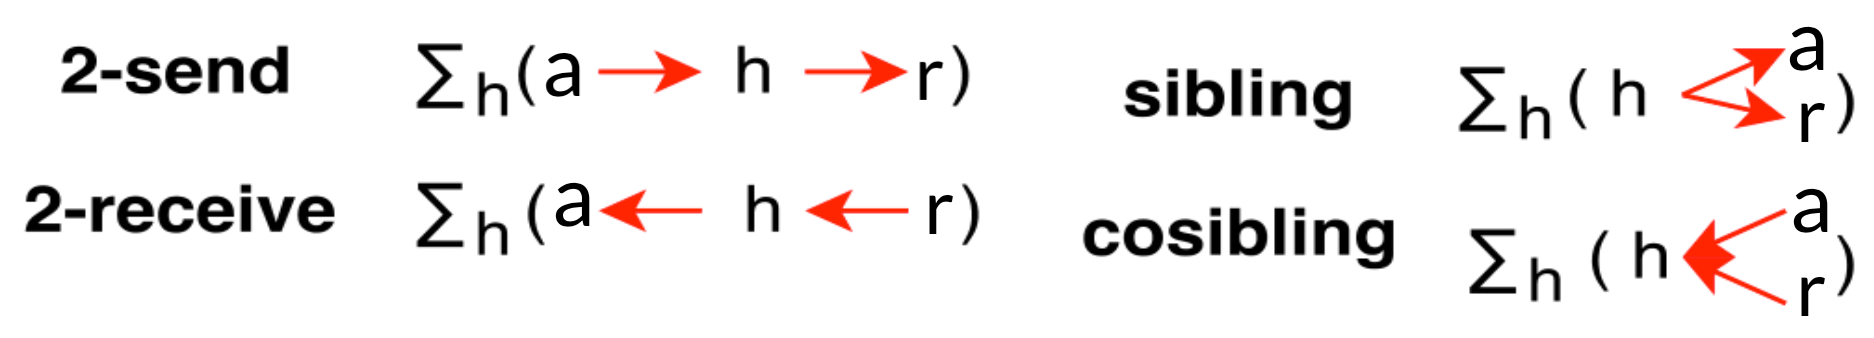
\includegraphics[width=0.6\textwidth]{img/triad-1.png}	
		\caption {Visualization of triadic statistics: 2-send, 2-receive, sibling, and cosibling.}
		\label{figure:netstats}
	\end{figure}
	
	\subsubsection{Timestamp covariates}
	For the event timing features $\boldsymbol{y}$ introduced in Section \ref{subsec:Time}, we identify a set of covariates which may effect ``time to the next email." Similar to the edge covariates, we include nodal statistics which are time-invariant (such as gender or manager status) or time-dependent (such as the network statistics used for $\boldsymbol{x}$). In addition, we select some edge-specific covariates based on the temporal aspect of the $(d-1)^{th}$ email---e.g., whether the previous email was sent (1) during the weekend and (2) before or past midday (AM/PM)---since we expect the email interactions within county government to be less active during the weekend and in the evening. To be specific, the timestamp statistics are defined as
	\begin{itemize}
		\item[1.] intercept: ${y}_{ad1} =1$;
		\item[2.] gender of sender: ${y}_{ad2}=I(\mbox{gender of sender }a= \mbox{female})$;
		\item[3.] manager status of sender: ${y}_{ad3}=I(\mbox{sender }a \mbox{ is the County Manager})$;
		\item[4.] outdegree of sender: ${y}_{ad4} =\sum_{d^\prime: t_{d^\prime} \in l_d} I(a_{d^\prime} = a)$;
		\item[5.] indegree of sender: ${y}_{ad5}=\sum_{d^\prime: t_{d^\prime} \in l_d} I(u_{d^\prime a} = 1)$;
		\item[6.] weekend indicator of previous email: ${y}_{ad6} = I(t_{d-1} \mbox{ is during the } \mbox{weekend})$;
		\item[7.] PM indicator of previous email: ${y}_{ad7}= I(t_{d-1} \mbox{ in } \mbox{PM})$.
	\end{itemize}
	Note that our generative process for timestamps in Section \ref{subsec:Time} is sender-oriented where the sender deterimes when to send the email, thus we incorporate network statistics that depends on $a$ only---outdegree of sender $a$ and indegree of sender $a$.
	
	\subsection{Model selection}\label{subsec:Experiment_email}
	
	The HEM has many component parts that need to be specified by the user (i.e., the receiver selection features $\boldsymbol{x}$, the selection of the event timing features $\boldsymbol{y}$, and the distribution of time increments $f$). Many of these components will be specified based on user expertise (e.g., regarding which features would drive receiver selection), but some decisions may require a data-driven approach to model specification. For example, though theoretical considerations may inform the specification of features, subject-matter expertise is unlikely to inform the decision regarding the family of the event time distribution. Furthermore, since different distribution families (and model specifications more generally) may involve different size parameter spaces, any data-driven approach to model comparison must guard against over-fitting the data. In this section we present a general-purpose approach to evaluating the HEM specification using out-of-sample prediction. We illustrate this approach by comparing alternative distributional families for the event timing component of the model. Here, we specifically compare the predictive performance from two distributions---log-normal and exponential. We particularly choose the log-normal distribution based on some exploratory analysis (e.g., histogram and simple regressions) on raw time increments data, and take exponential distribution as an alternative since exponential is the most commonly specified distribution for time-to-event data, and is also used in the stochastic actor-oriented models (SAOMs) \citep{snijders1996stochastic} as well as their extensions \citep{snijders2007modeling}. 
	\begin{algorithm}[!t]
		\spacingset{1}
		\caption{Out-of-Sample Predictions}
		\label{alg:PPE}
		\begin{algorithmic}
			\STATE {\bfseries Input}: data $ \{ (a_d, \boldsymbol{r}_d, t_d)\}_{d=1}^D$, 
			number of new data to generate $R$, and initial values of $(\boldsymbol{b}, \boldsymbol{\eta}, \boldsymbol{u}, \sigma^2_\tau)$
			\vskip 0.1in
			\textbf{Test splits} (with $p=0.1$):	
			\STATE draw test senders (out of $D$ senders) 
			\STATE draw test receivers (out of $D\times (A-1)$ receiver indicators $\{\{\boldsymbol{r}_{dr}\}_{r\in [A]_{\backslash a_d}}\}_{d=1}^D$)
			\STATE draw test timestamps  (out of $D$ timestamps) 
			\STATE set the test data as ``missing" (NA)
			\vskip 0.1in
			\textbf{Imputation and inference:}	
			\FOR{$r=1$ {\bfseries to}  $R$}
			\FOR{$d=1$ {\bfseries to}  $D$}
			\IF{$a_d=$  NA}
			\FOR{$a=1$ {\bfseries to} $A$}
			\STATE compute $\pi_{a}=P(a_d= a | \cdot)$ using equation (\ref{eqn:latenttime}) (without the product term)
			\ENDFOR
			\STATE draw $a_d \sim \mbox{multinomial}(\pi_a)$
			\ENDIF
			\FOR{$r\in [A]_{\backslash a_d}$}
			\IF{$r_{dr}=$ NA}
			\STATE draw $r_{dr}$ from multinomial with probability $P(r_{dr}= 1 | \cdot)$ and $P(r_{dr}= 0| \cdot)$ using equation (\ref{eqn:latentreceiver})
			\ENDIF
			\ENDFOR
			\IF{$t_d=$ NA}
			\STATE draw $\boldsymbol{\tau}^{new}_d$ from equation (\ref{eqn:latenttime}) (without the product term) via importance sampling\footnote{we need to specify appropriate proposal distribution such as $g \sim \mbox{halfcauchy}(5)$}
			\ENDIF
			\STATE run inference and update $(\boldsymbol{u},\boldsymbol{b}, \boldsymbol{\eta})$ given the imputed and observed data
			\ENDFOR
			\STATE store the estimates for test data
			\ENDFOR
		\end{algorithmic}
	\end{algorithm}
	
	We evaluate the model's ability to predict edges and timestamps from Montgomery County email data, conditioned on their ``training" part of the data. To perform the experiment, we separately formed a test split of each three model components---sender, receivers, and timestamps---by randomly selecting ``test" data with probability $p=0.10$, and setting the test data to missing. Any missing variables were imputed by drawing samples from their conditional posterior distributions, given the observed data, model estimates, and current values of imputed test data. We then run inference to update the latent variables given the imputed and observed data. We iterate the two steps---imputation and inference---multiple times to obtain posterior samples of the held out test data. Algorithm \ref{alg:PPE} outlines this procedure in detail. We run the experiment and measure the predictive performance of two separate time distributions using $N=500$ predicted samples, by comparing the predictions in terms of classification accuracy in predicting the senders and receivers, as well as prediction error in the timestamps. We summarize the results of prediction experiments for missing senders, receivers, and timestamps in Figure \ref{figure:PPEresults}. First, we compare the posterior probability of correct senders for each of the missing emails $\{d:a_d=\mbox{NA}\}$, which corresponds to $\pi_{a_{d}}=P(a_{d} = a^{obs}_{d}|\cdot)$ in Algorithm \ref{alg:PPE}. We call this measure the ``correct sender posterior probability." On Figure \ref{figure:PPEresults} (a), we draw boxplots for the distribution of mean correct sender posterior probability---i.e., $\hat{\pi}_{a_{d}} = \frac{1}{N}\sum_{n=1}^N \pi^n_{a_{d}}$---across the missing emails. The results show that both log-normal and exponential distributions acheive better predictive performance for missing senders compared to what is expected under random guess (i.e., choose one out of $A$ possible senders $=1/18$), with log-normal distribution showing higher performance than exponential distribution. Secondly, since the receiver vector is binary, we compute $F_1$ scores for missing receiver indicators (i.e., all $d$ and $r$ with $r_{dr}$=NA) by taking the harmonic mean of precision and recall:
	\begin{equation}
		\begin{aligned}
			F_1 =2\cdot\frac{\mbox{precision}\cdot \mbox{recall}}{\mbox{precision}+ \mbox{recall}}, &\mbox{ where } \\
			\mbox{recall}  = \frac{\mbox{TP}}{\mbox{TP+FN}} \mbox{ and } \mbox{precision} & =\frac{\mbox{TP}}{\mbox{TP+FP}},
		\end{aligned}
	\end{equation}
	with TP denoting true positive (i.e., $\boldsymbol{r}^{obs}_{dr}=\boldsymbol{r}^{pred}_{dr}=1$), FN denoting false negative (i.e., $\boldsymbol{r}^{obs}_{dr}=1$ but $\boldsymbol{r}^{pred}_{dr}=0$), and FP denoting false positive (i.e., $\boldsymbol{r}^{obs}_{dr}=0$ but $\boldsymbol{r}^{pred}_{dr}=1$). Although the generative process for edges (Section \ref{subsec: Tie}) is not directly affected by the choice of timestamp distribution, Figure \ref{figure:PPEresults} (b) reveals slight difference between log-normal and exponential in their performance in predicting missing receiver indicators, where log-normal on average outperforms exponential. Finally, the prediction error for $d^{th}$ missing timestamp is estimated using the median of absolute relative errors\footnote{\cite{hyndman2006another} refer to this as median absolute percentage error (MdAPE).} across $N=500$ predictions:
	\begin{figure}[!t]
		\centering
		\begin{tabular}[t]{ccc}
			\begin{subfigure}[b]{0.33\textwidth}
				\caption{Sender prediction}
				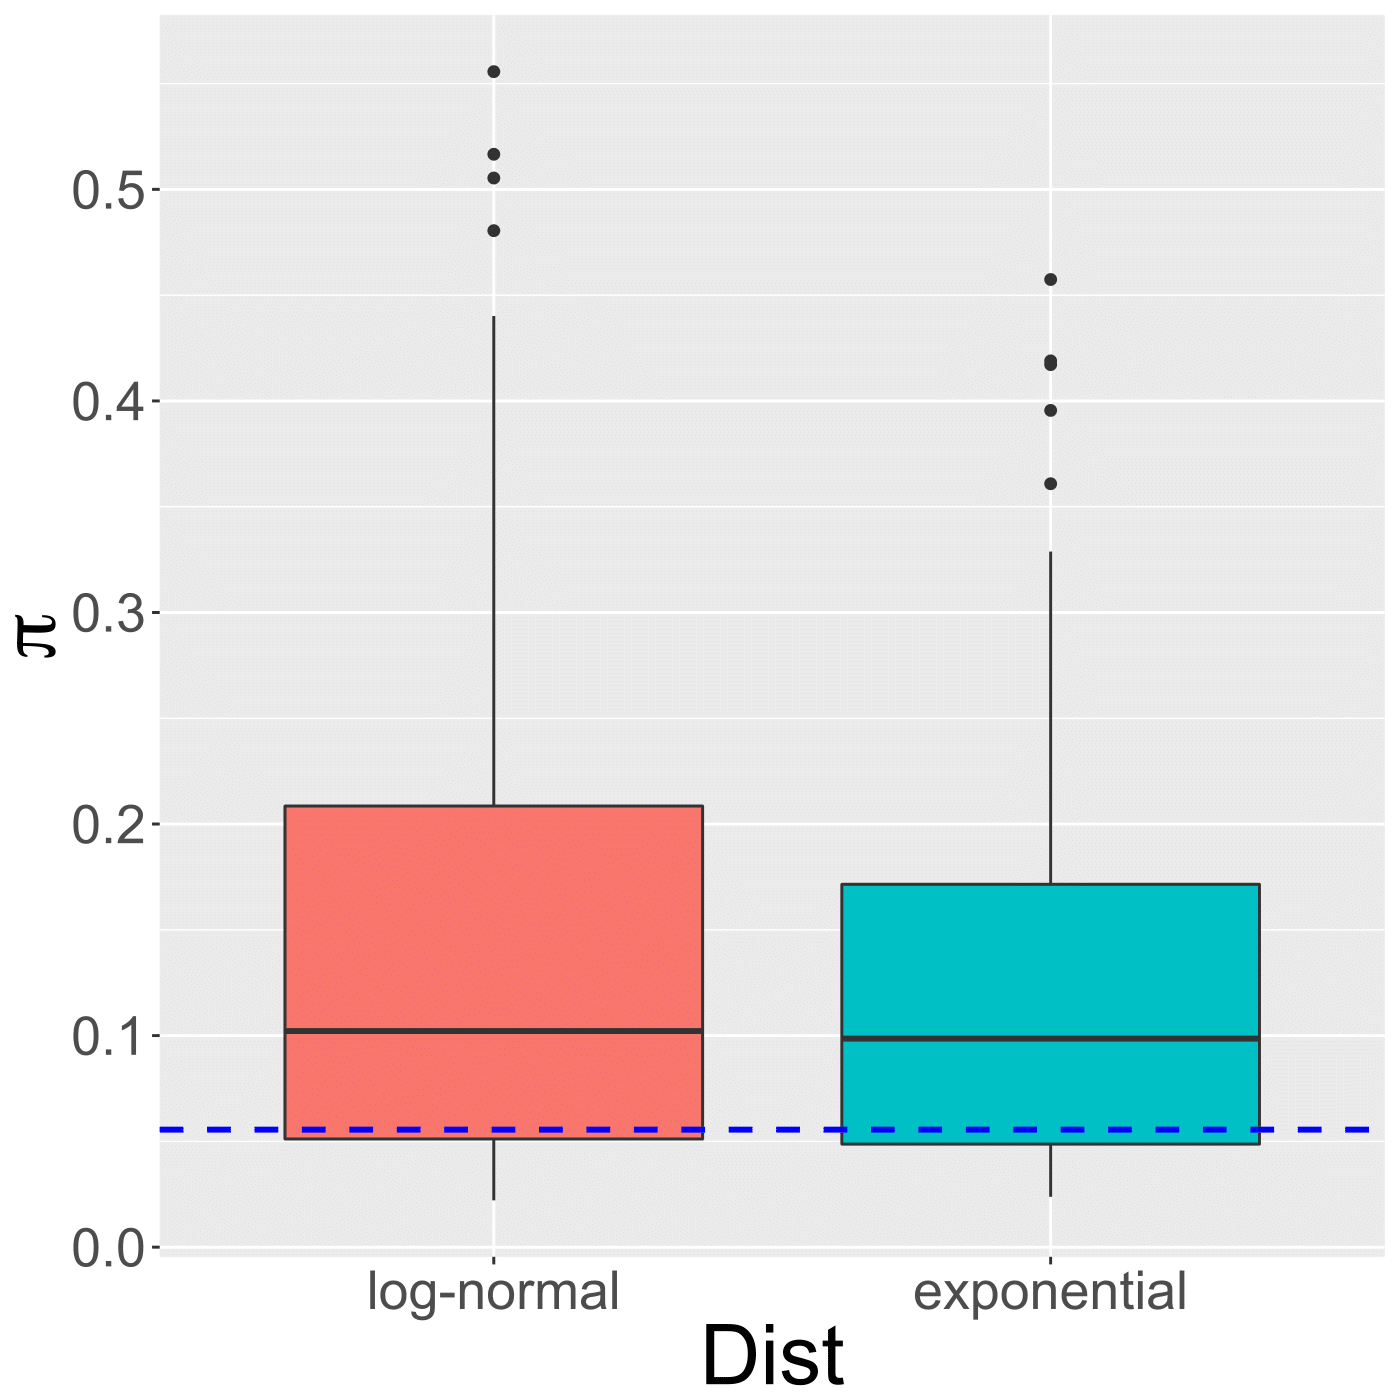
\includegraphics[width=\textwidth]{img/senderpredict-1.png}	
			\end{subfigure}
			\begin{subfigure}[b]{0.33\textwidth}
				\caption{Receiver prediction}
				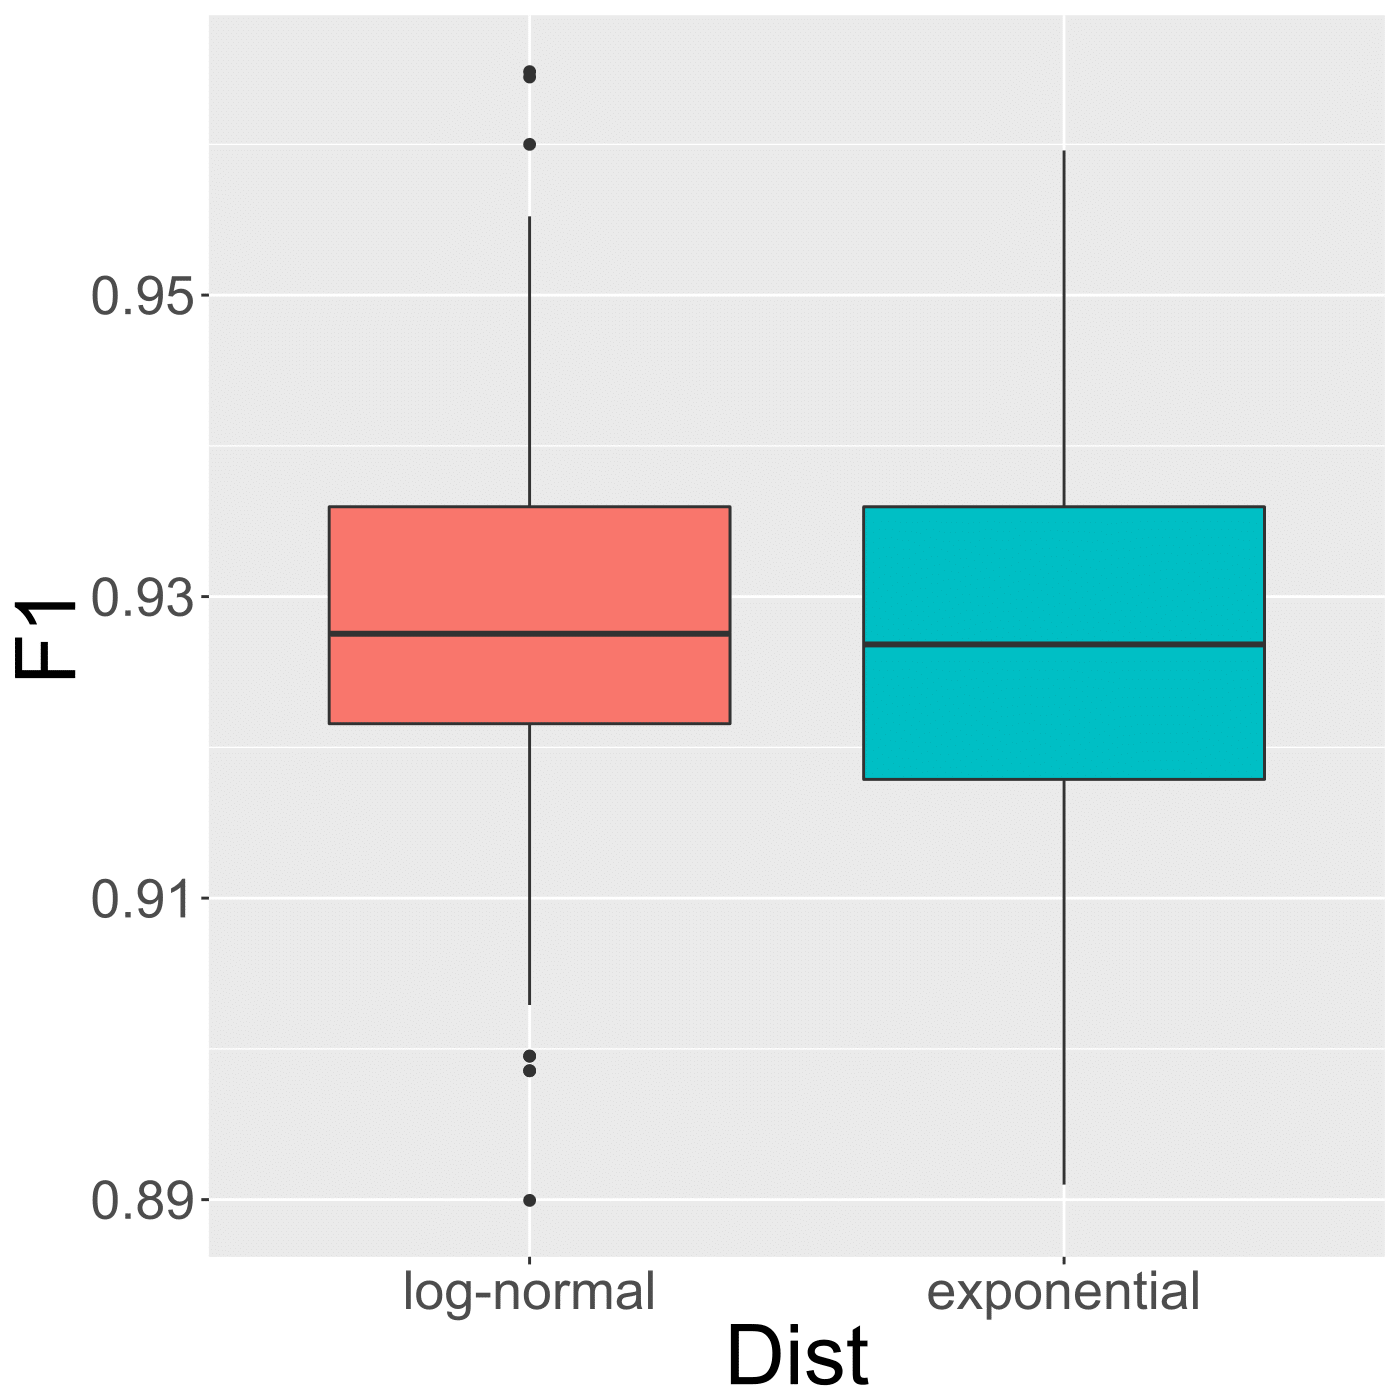
\includegraphics[width=\textwidth]{img/receiverpredict-1.png}	
			\end{subfigure}
			\begin{subfigure}[b]{0.33\textwidth}
				\caption{Timestamp prediction}
				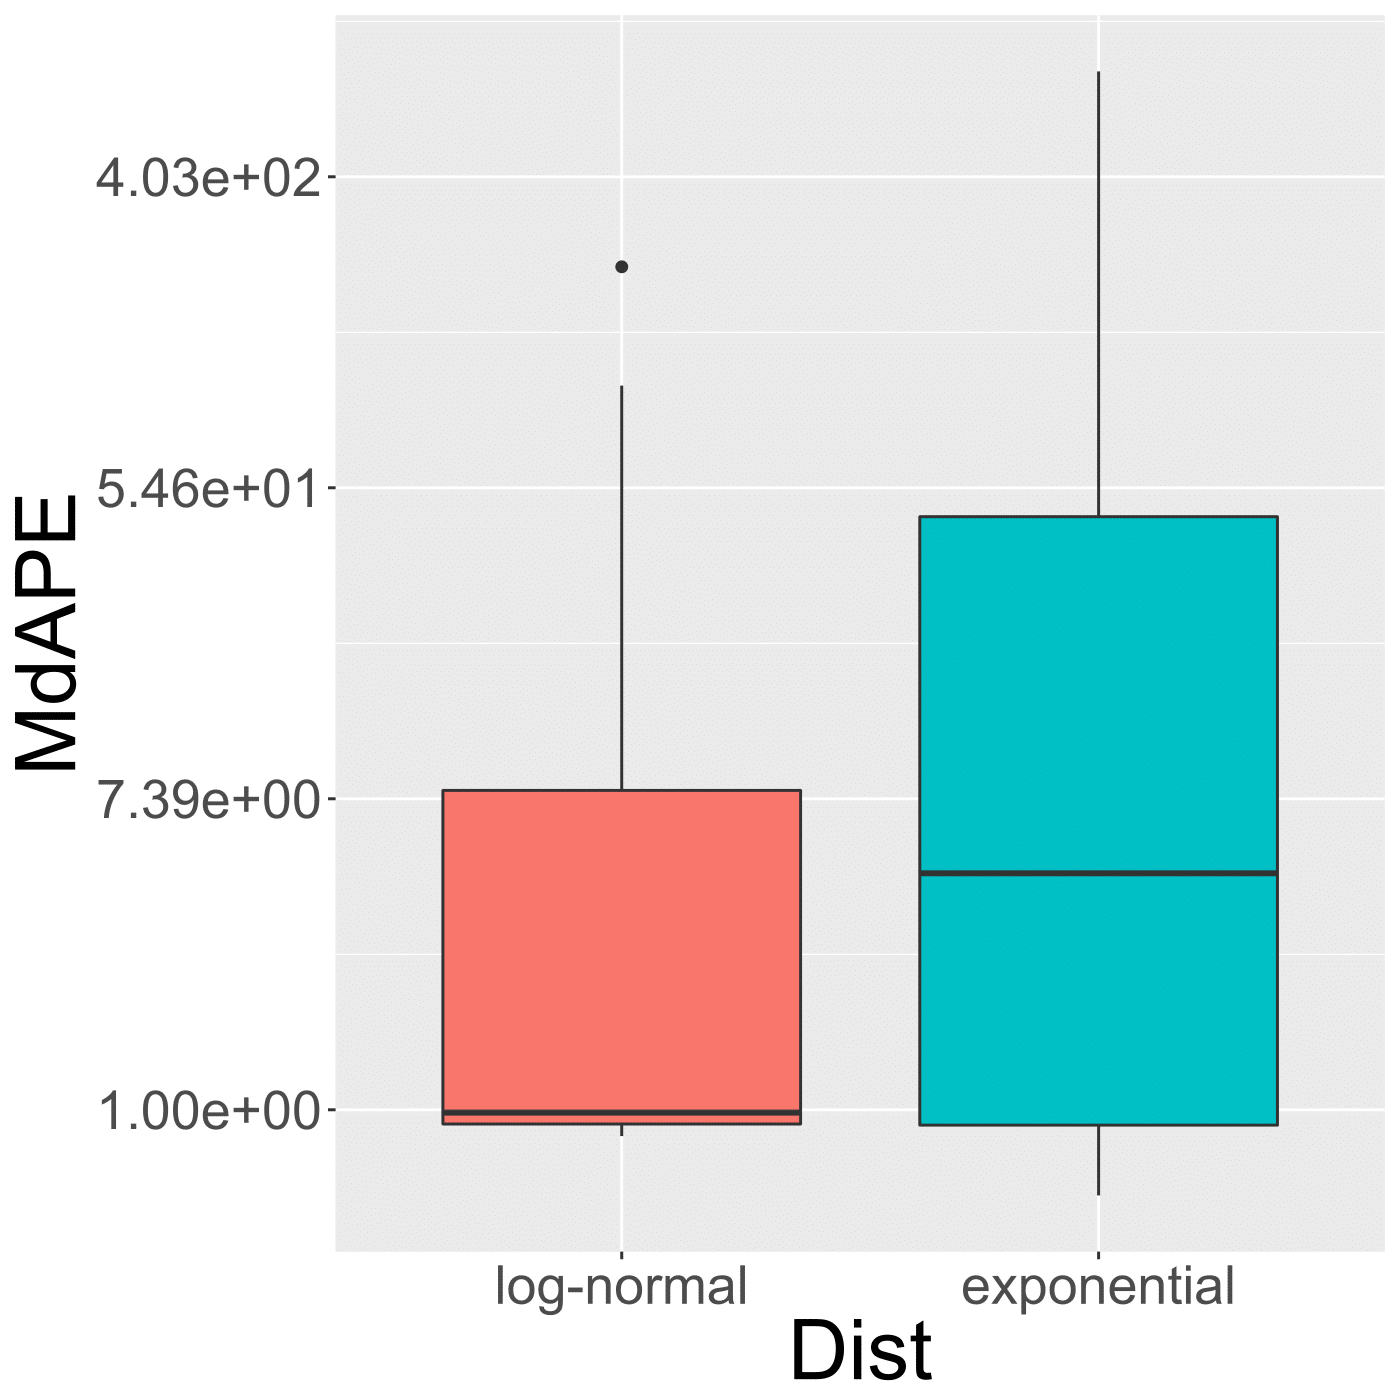
\includegraphics[width=\textwidth]{img/timepredict-1.png}	
			\end{subfigure}
		\end{tabular}
		
\includegraphics[width=0.4\textwidth]{img/modellabel.png}				
		\caption {Comparison of predictive performance between log-normal and exponential distributions: (a) correct sender posterior probability from sender predictions, (b) $F_1$ scores from receiver predictions, and (c) median absolute relative error from timestamp predictions. Blue line in (a) represents the correct sender probability expected by random guess---i.e., $1/A=1/18\approx0.056$.}
		\label{figure:PPEresults}
	\end{figure}		
	\iffalse
	\begin{figure}[!t]
		\centering
		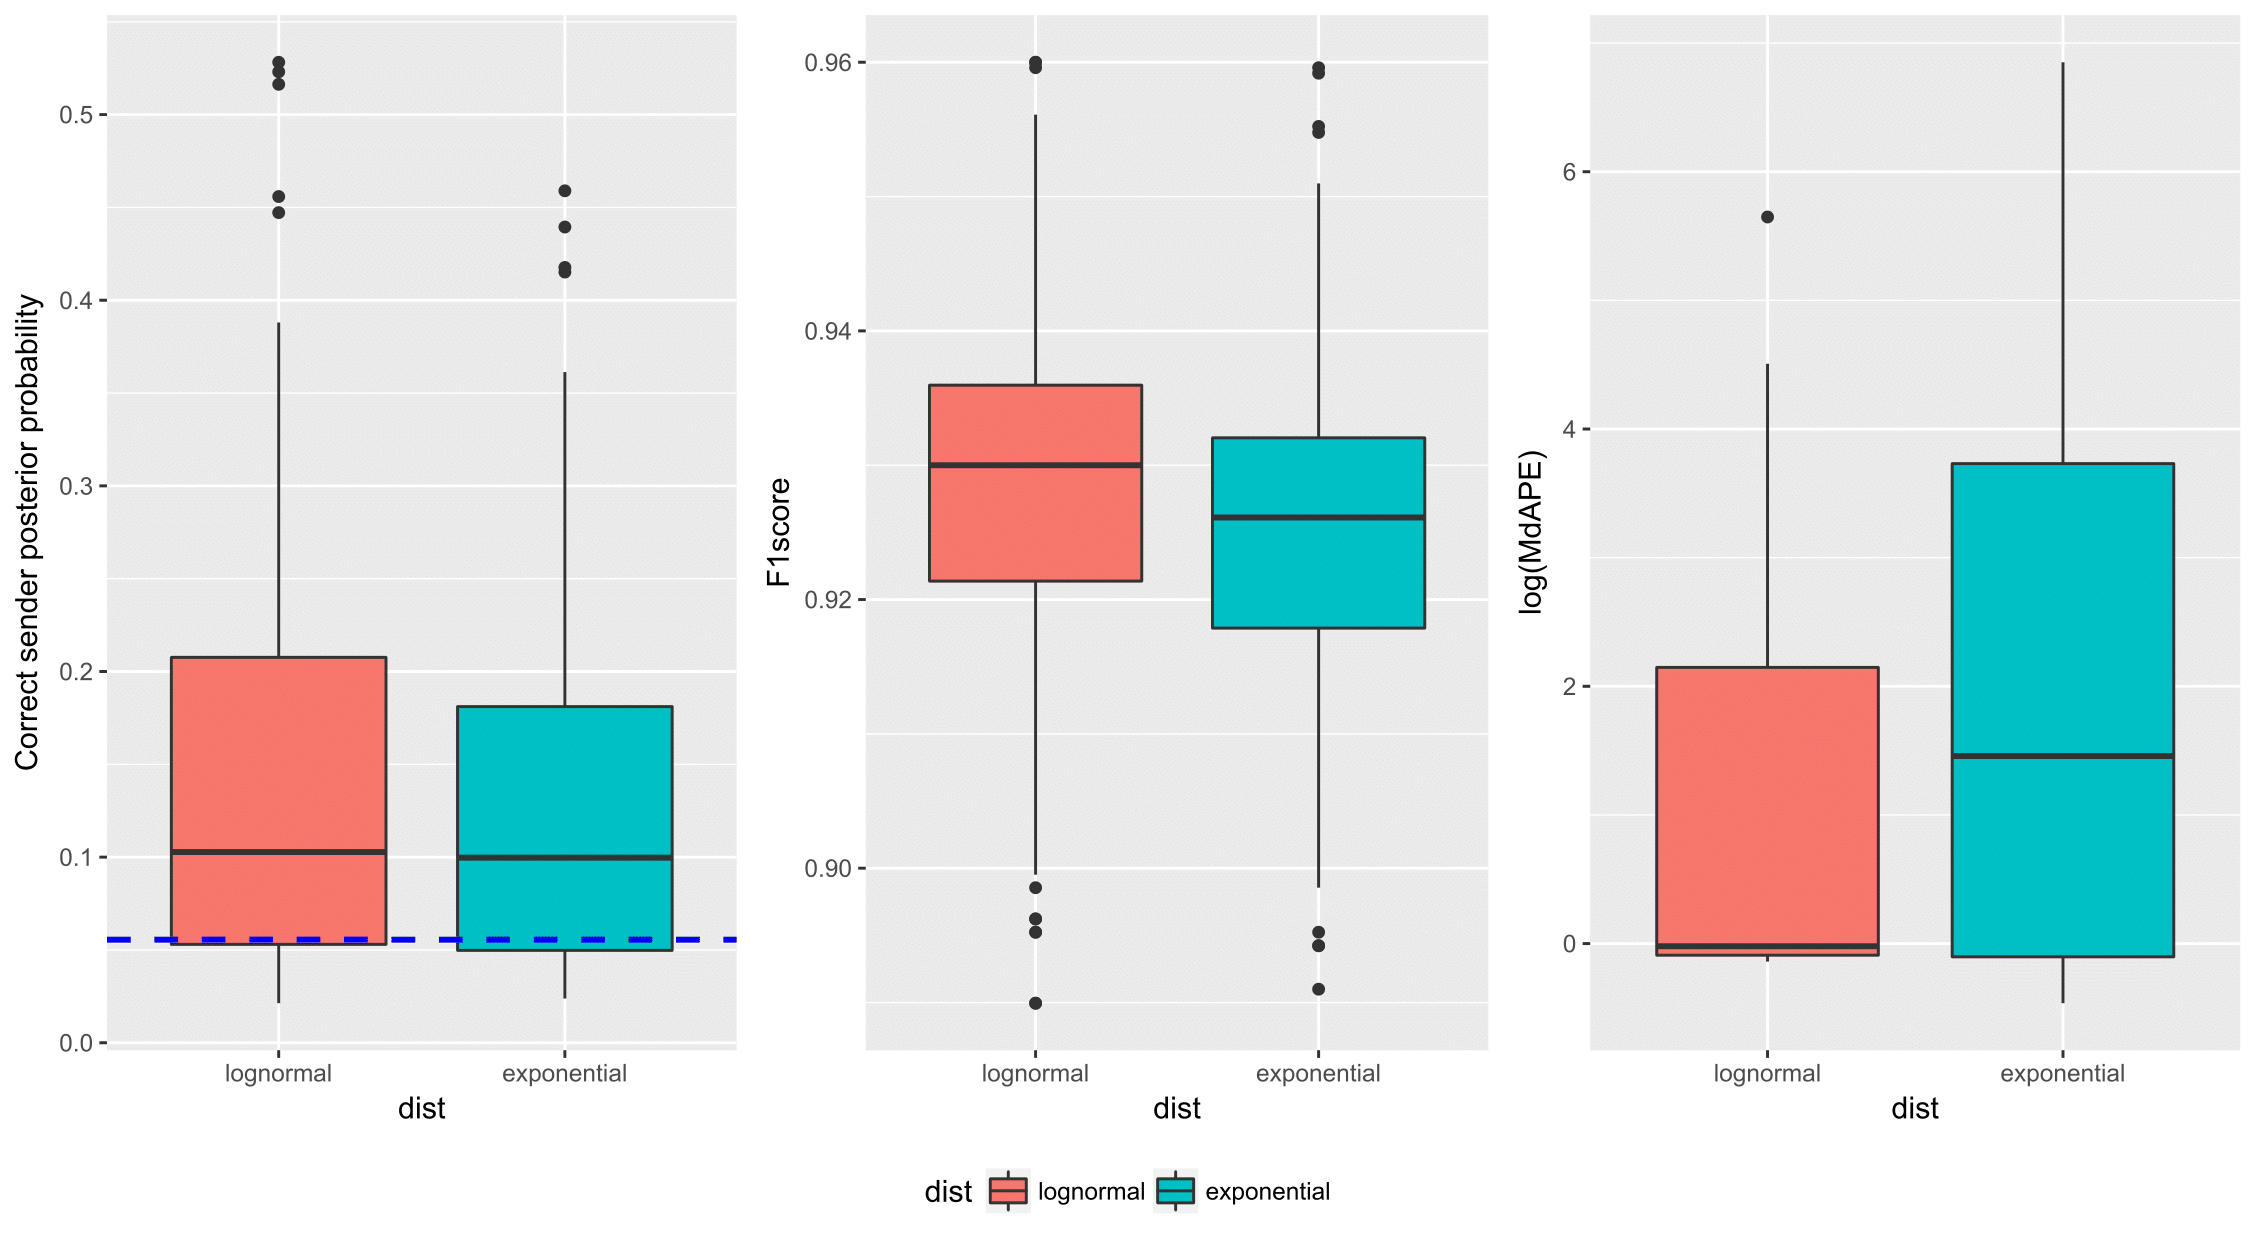
\includegraphics[width=1\textwidth]{img/PPEplotnew-1.png}	
	\end{figure}
	\fi
	\begin{equation}
		e_{\tau_d} = \mbox{median}\Big(\abs*{\frac{\tau^{obs}_d - \tau^{pred_1}_{d}}{\tau^{obs}_d}},\ldots, \abs*{\frac{\tau^{obs}_d - \tau^{pred_N}_{d}}{\tau^{obs}_d}}\Big).
	\end{equation}
	Figure \ref{figure:PPEresults} (c) presents boxplots for the median absolute relative errors. where plot the estimates in a log-scale. Surprisingly, we have a huge benefit in the performance of timestamp prediction when we assume log-normal distribution for time-increments compared to exponential distribution. This difference can be explained by overdispersion in exponential distribution, because there exists greater variability in the time increments of emails than would be expected under exponential distribution. As illustrated above, we can use this out-of-sample prediction task for two uses---1) to provide an effective answer to the question ``how does the HEM perform at filling in the missing components of time-stamped network data?" and 2) to offer one standard way to determine the distribution of time increments in Section \ref{subsec:Time}. 
	
	\subsection{Posterior predictive checks}\label{subsec:PPC_email} 	   
	In this section, we perform posterior predictive checks (PPC) \citep{rubin1984bayesianly} to evaluate the appropriateness of our model specification for Montgomery County email data. We formally generated entirely new data by simulating $N=500$ synthetic email datasets $\{(a_{d}, \boldsymbol{r}_{d}, t_{d})\}_{d=1}^D$ from the generative process in Section \ref{sec:generative process}, conditional upon a set of inferred latent variables from the inference in Section \ref{subsec:Result_email}\iffalse, where the pseudocode is outlined in Algorithm \ref{alg:PPC}\fi. For the test of goodness-of-fit in terms of network dynamics, we use multiple statistics that summarize meaningful aspects of the data: outdegree distribution---the number of edges sent by each node, indegree distribution---the number of edges received by each node, receiver size distribution---the number of receivers on each edge, and a probability-probability (PP) plot for time increments. 
	\iffalse
	\begin{algorithm}[!t]
		\spacingset{1}
		\caption{Generate new data for PPC}
		\begin{algorithmic}
			\STATE \textbf{Input}: number of data to generate $R$, covariates $(\boldsymbol{x},\boldsymbol{y})$, and estimated values of $(\boldsymbol{u}, \boldsymbol{b}, \boldsymbol{\eta})$\\
			\vskip 0.1in
			
			\FOR{$r=1$ {\bfseries to}  $R$}
			\FOR{$d = 1$ {\bfseries to}  $D$} 
			\STATE	Draw ($a_{d}$, $\boldsymbol{r}_{d}$, $t_{d}$) following Algorithm \ref{alg:generative}\\
			\ENDFOR
			\STATE Store every $r^{th}$ new data $\{(a_{d}, \boldsymbol{r}_{d}, t_{d})\}_{d=1}^D$ 
			\ENDFOR
		\end{algorithmic}
		\label{alg:PPC}
	\end{algorithm}     \fi  
	\begin{figure}[!t]
		\centering
		\begin{tabular}[t]{cc}
			\begin{subfigure}[b]{0.495\textwidth}
				\caption{Outdegree distribution}
				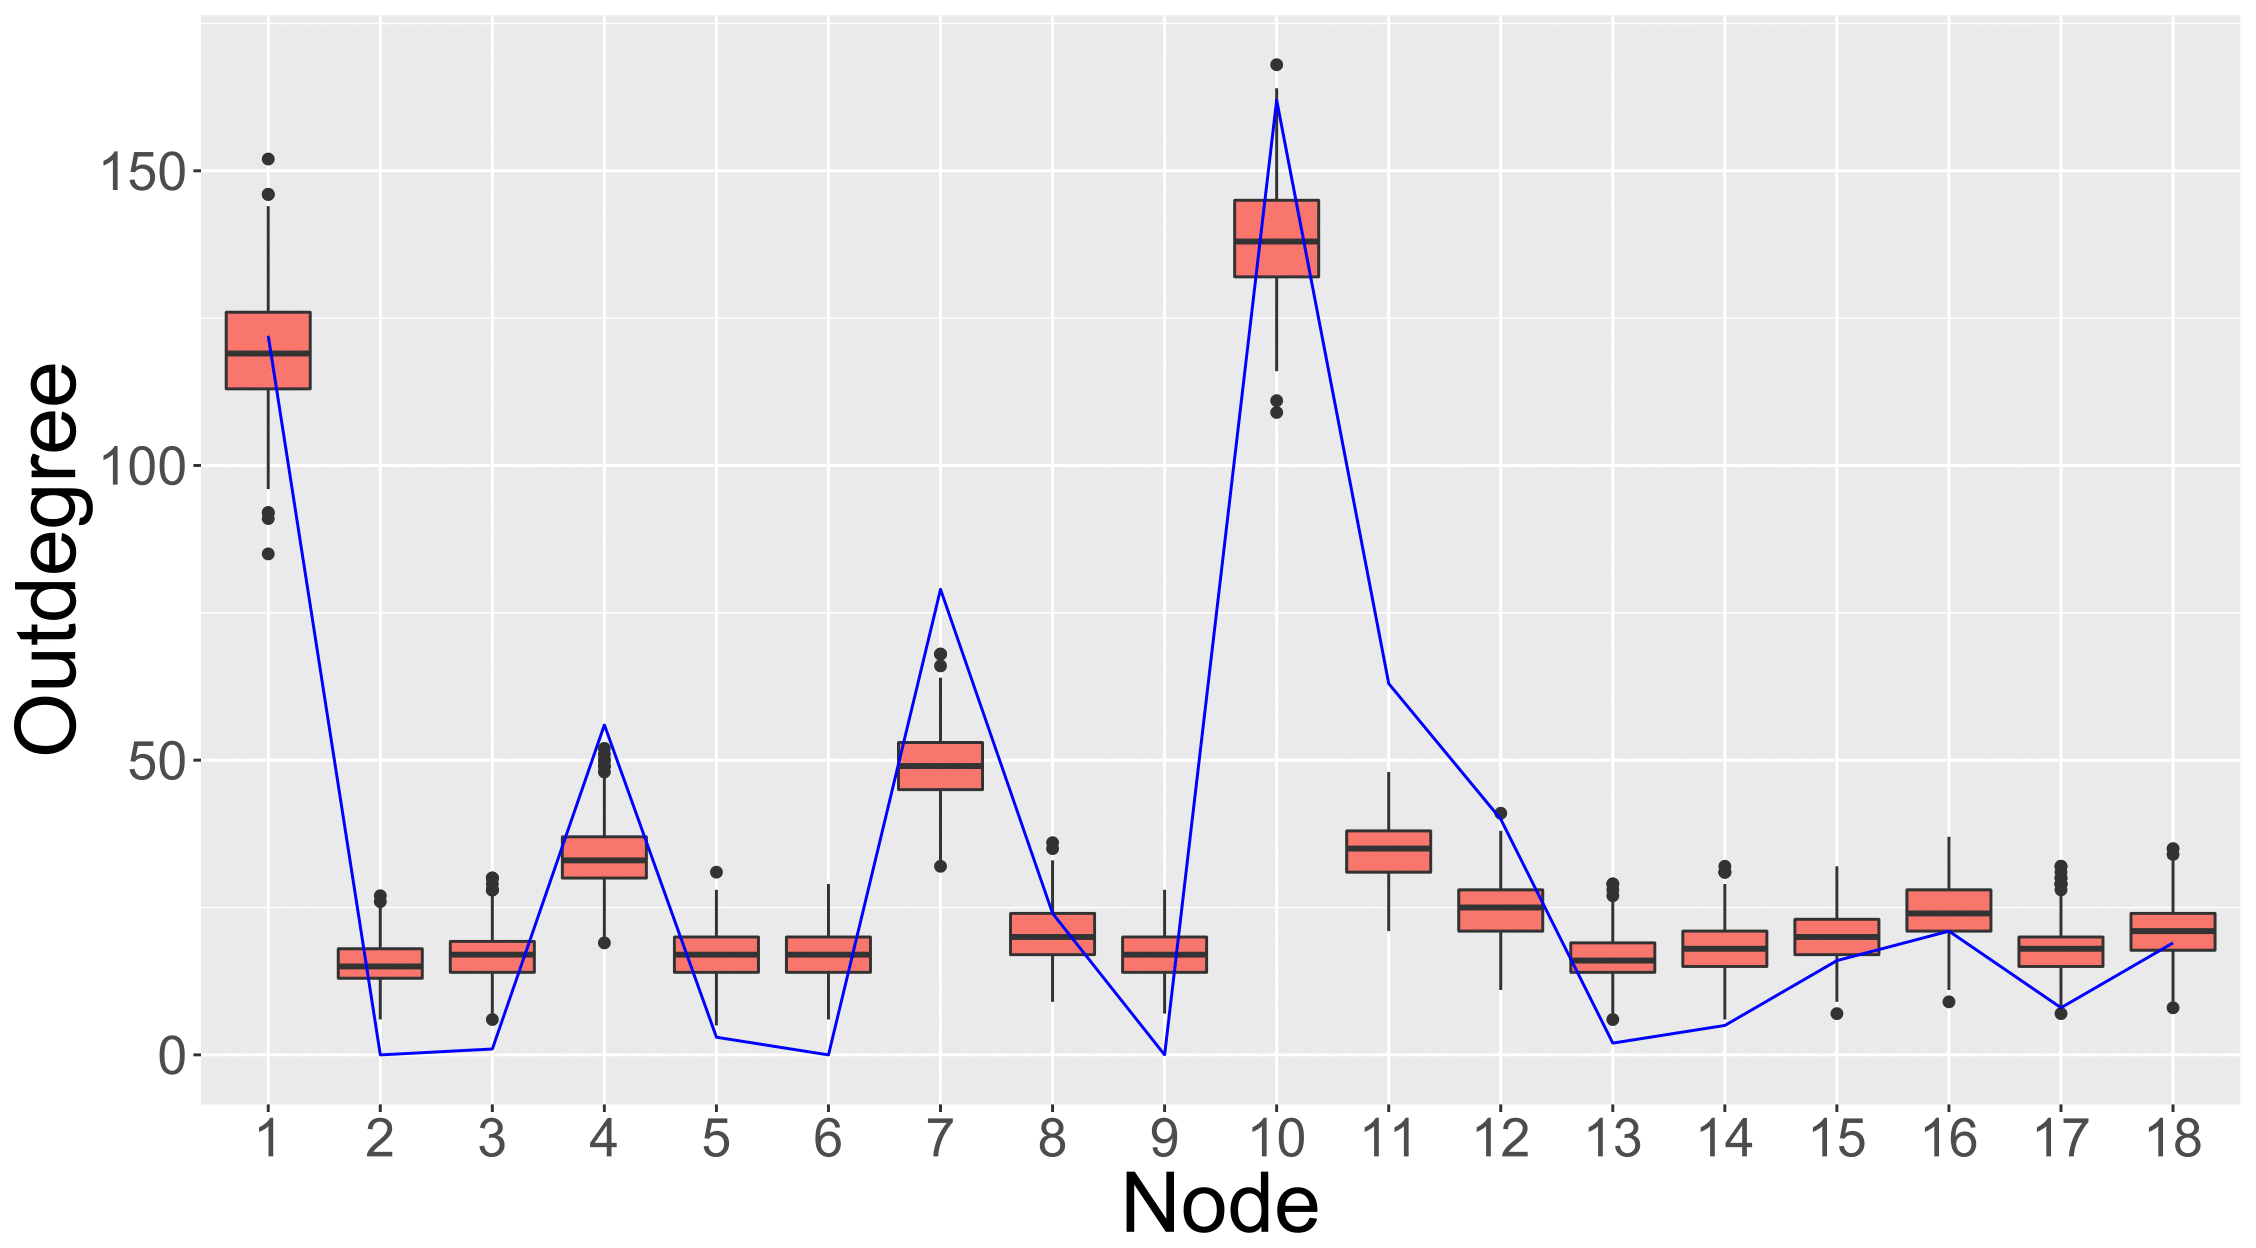
\includegraphics[width=\textwidth]{img/outdegree-1.png}	
			\end{subfigure}
			\begin{subfigure}[b]{0.495\textwidth}
				\caption{Indegree distribution}
				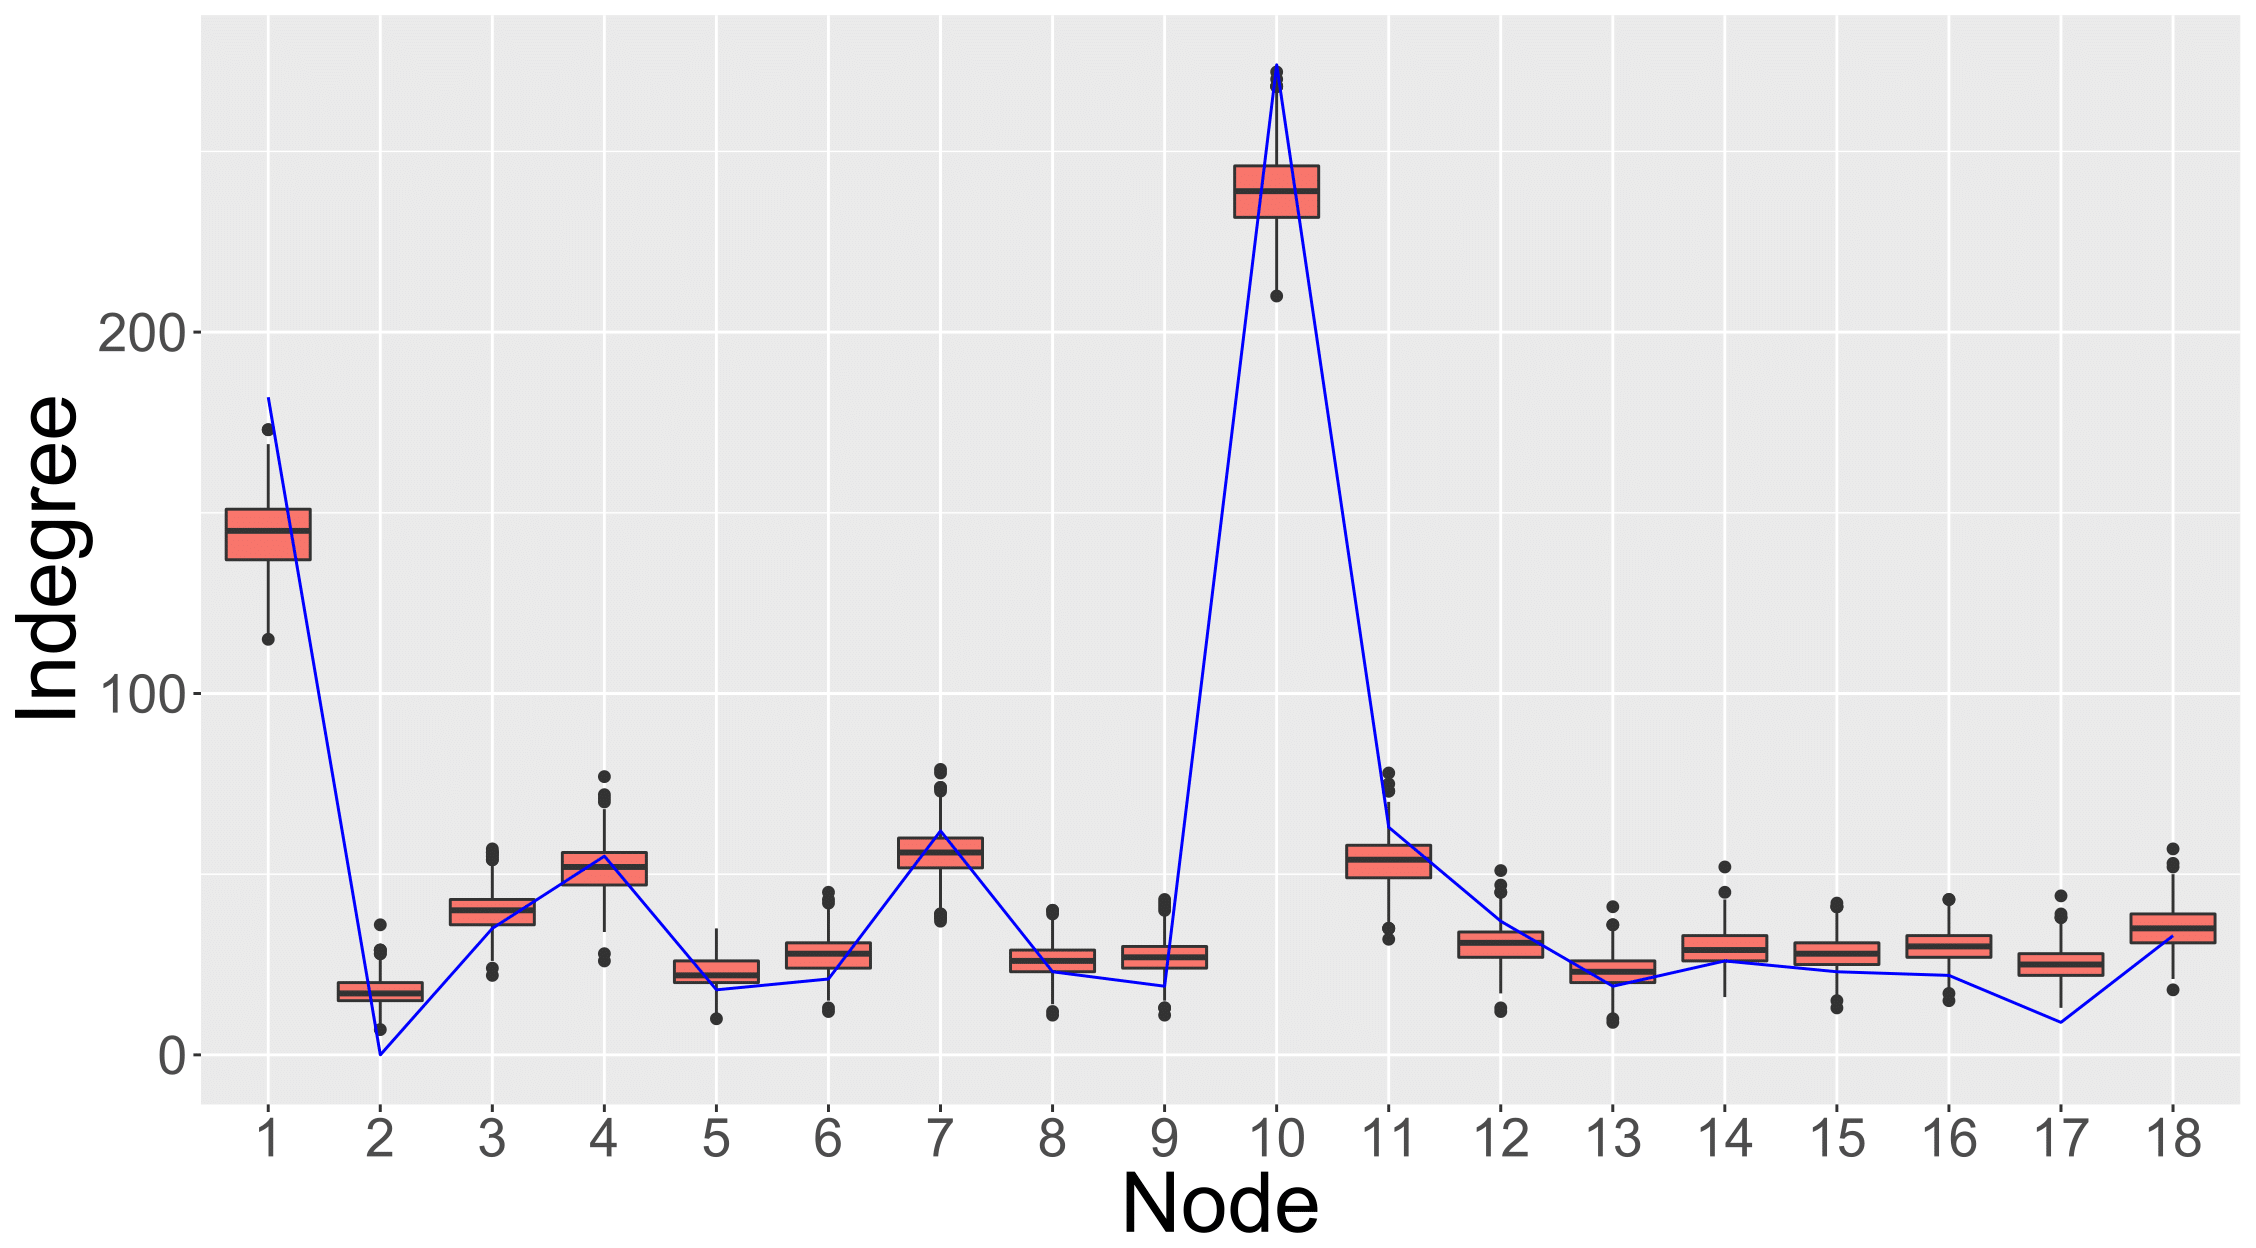
\includegraphics[width=\textwidth]{img/indegree-1.png}	
			\end{subfigure}\\
			\begin{subfigure}[b]{0.495\textwidth}
				\caption{Receiver size distribution}
				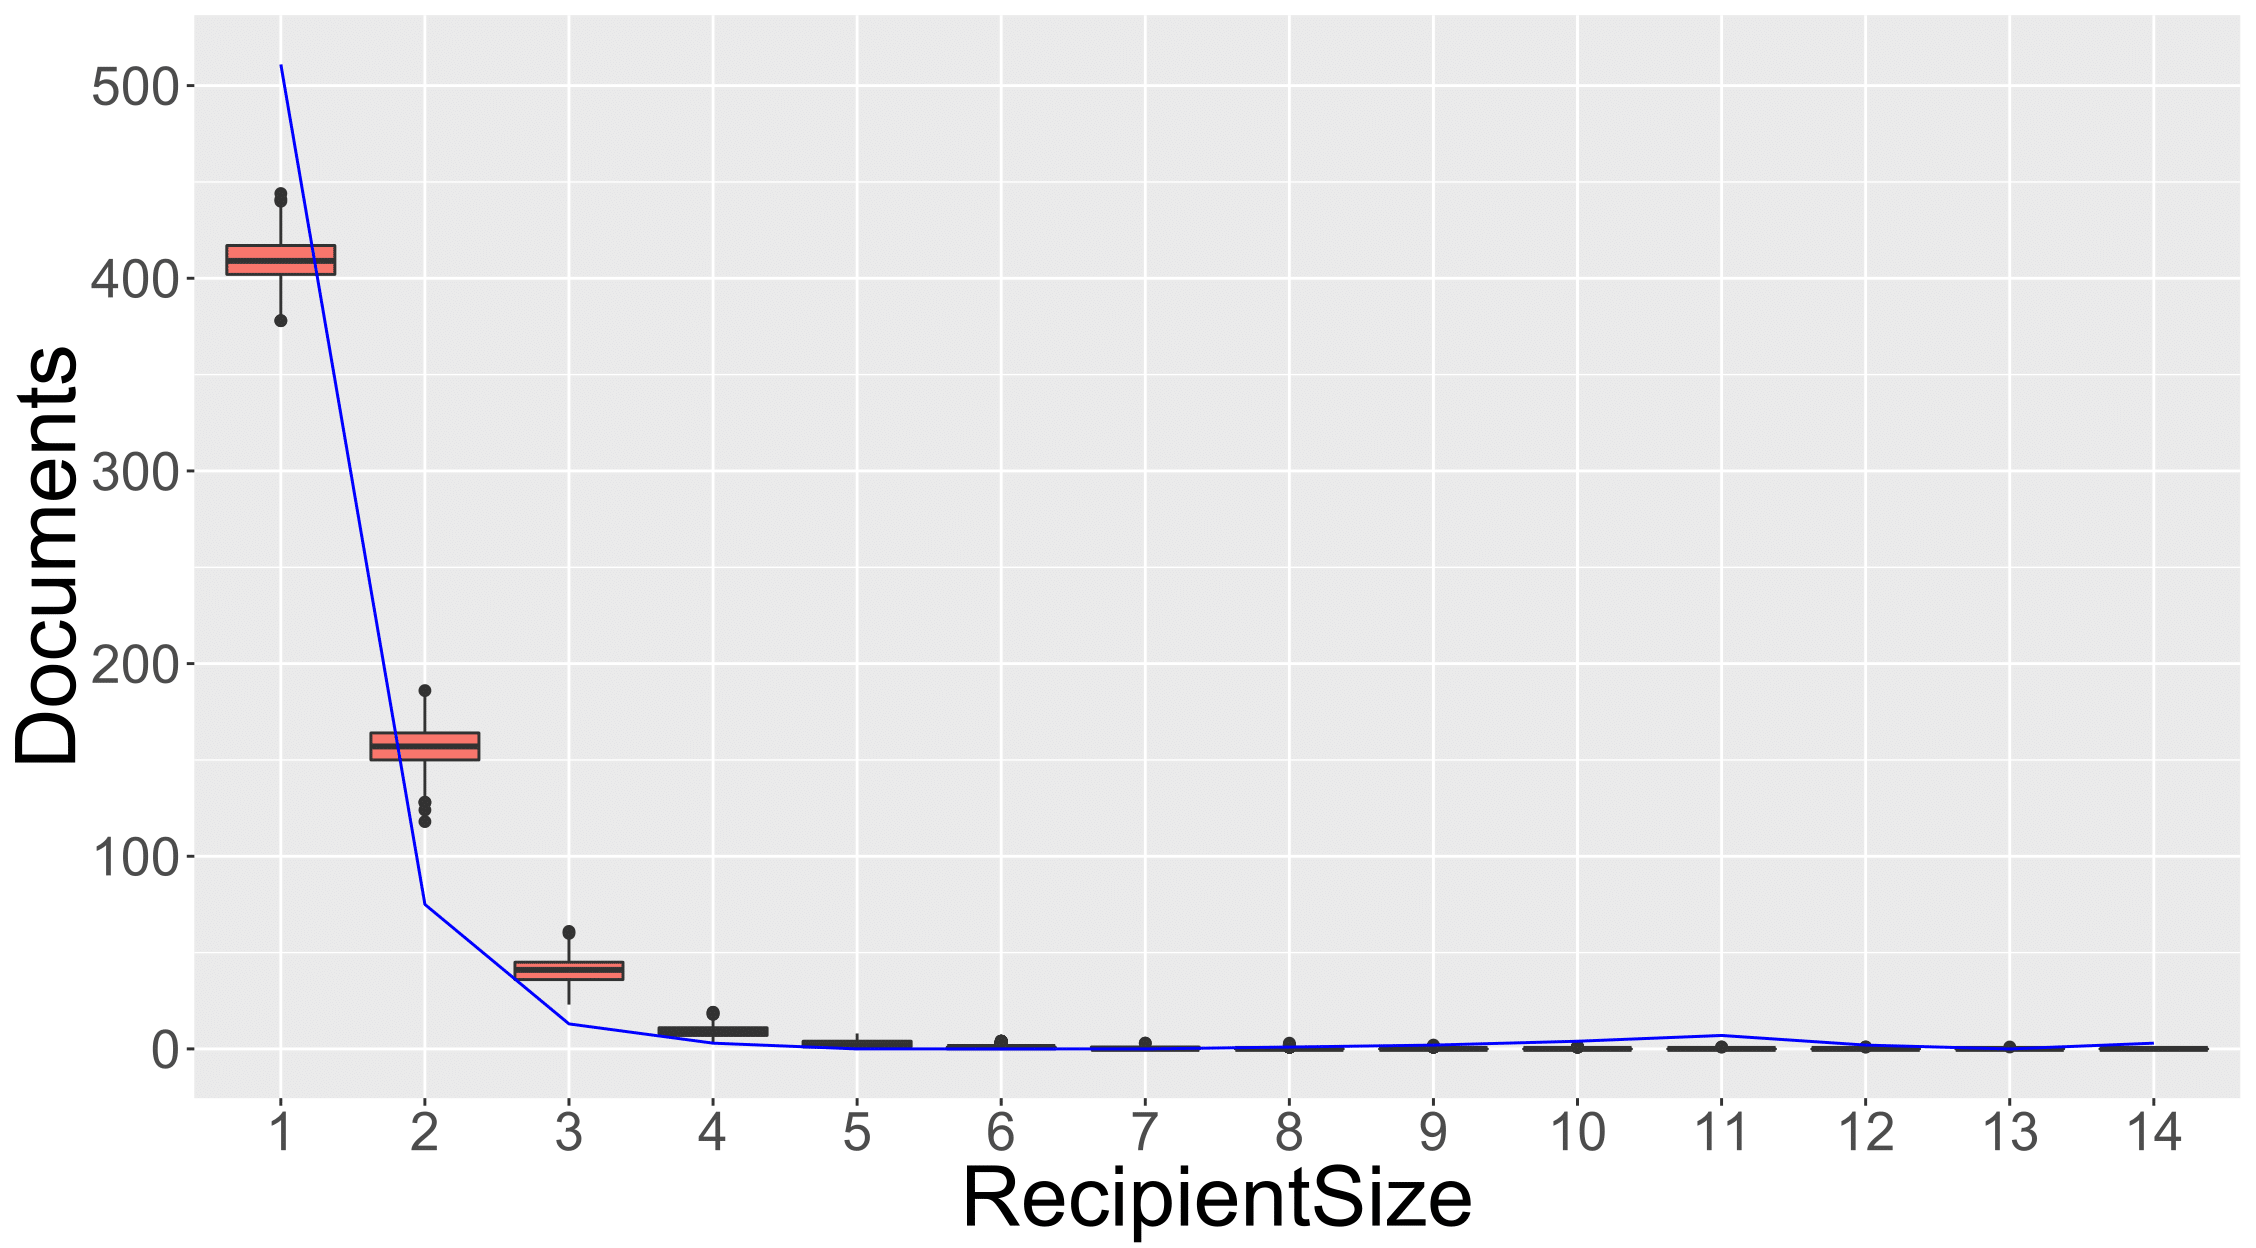
\includegraphics[width=\textwidth]{img/recipientsize-1.png}	
			\end{subfigure}
			\begin{subfigure}[b]{0.495\textwidth}
				\centering
				\caption{PPplot for time increments}
				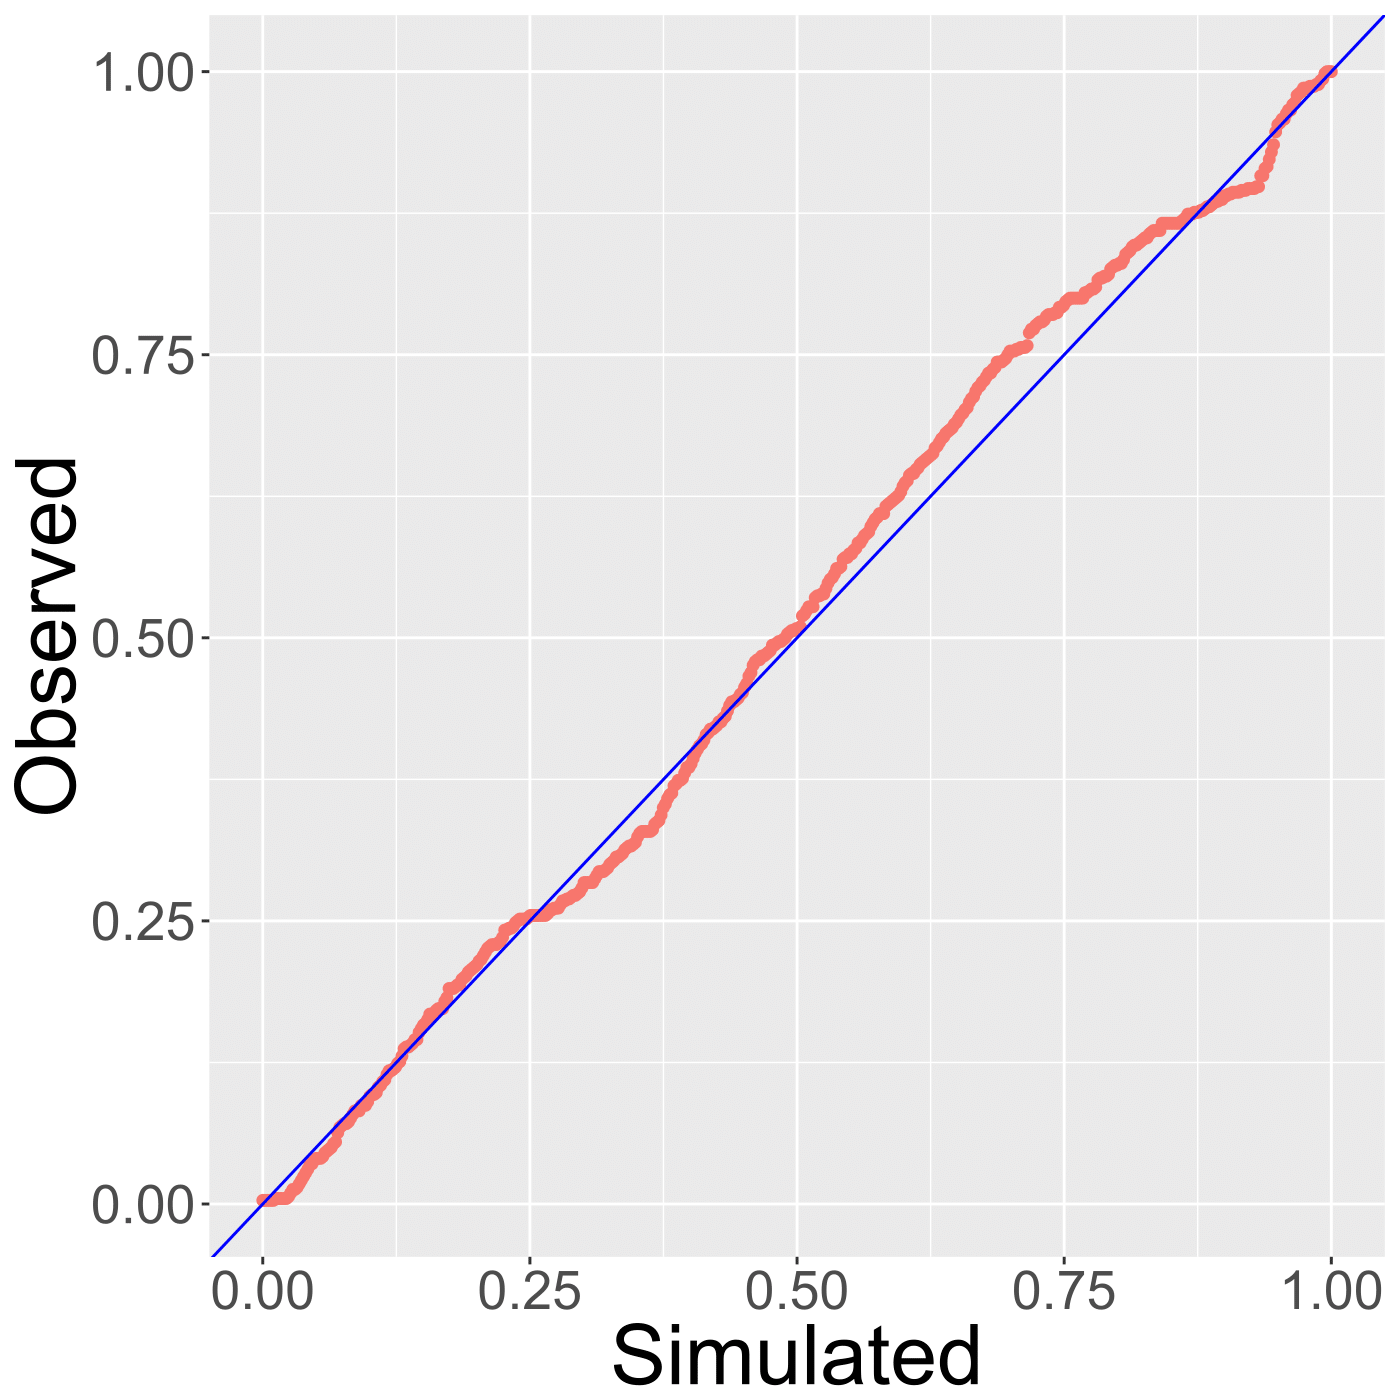
\includegraphics[width=0.56\textwidth]{img/timePPplot-1.png}	
			\end{subfigure}
		\end{tabular}
		\caption {PPC results from log-normal distribution. Blue lines denote the observed statistics in (a)--(c) and denotes the diagonal line in (d).}
		\label{figure:PPCresults}
	\end{figure}
	
	Figure \ref{figure:PPCresults} illustrates the results of poterior predictive checks using the log-normal distribution, which shows better performance in Section \ref{subsec:Experiment_email}. The upper two plots show node-specific posterior predictive degree distributions across $N=500$ synthetic samples, where the left one for outdegree statistic and the right plot is for indegree statistic. For both plots, the x-axis represents the nodes ($A=1,\ldots,18$), and the y-axis represents the number of emails sent or received by the node. When compared with the observed outdegree and indegree statistics (red lines), our model recovers the overall distribution of sending and receiving activities across the nodes. For example, node 1 and 10 show significantly higher level of both sending and receiving activities relative to the rest, and the model-simulated data captures those big jumps, showing acceptable fit to the data. Outdegree distribution of some low-activity nodes are not precisely recovered, however, indegree distribution looks much better. Since we use more information in the receiver selection process (i.e., network effects) while we rely solely on minimum time increments when choosing the observed sender, these results are expected. The lower left plot is the distribution of receiver sizes, where the x-axis spans over the size of receivers 1 to 14 (which is the maximum size of observed receivers) and the y-axis denotes the number of emails with x-number of receivers. The result shows that our model is underestimating emails with one receiver while overestimating emails with two, three, and four receivers. One explanation behind what we observe is that the model is trying to recover so-called ``broadcast'' emails, which are the emails with $\geq 10$ number of receivers, so that the intercept estimate $b_1$ is slightly moved toward right. It would be an interesting problem in future research to consider how the hyperedge size distribution can be further modified to capture this distribution more accurately. The plot on the lower right is the PP plot for time increments, which depicts the two cumulative distribution functions---one for simulated time increments and another for observed time increments---against each other in order to assess how closely two data sets agree. Here, the closeness to the diagonal line connecting $(0, 0)$ and $(1, 1)$ gives a measure of difference between the simulated and observed time increments, and our PP plot shows that we have great performance in reproducing the observed time distribution. Our findings from the predictive experiments in Section \ref{subsec:Experiment_email} are further revealed in the PPC from exponential distribution, where the PPC plots comparing log-normal and exponential distributions are presented in Appendix C.
	
	\subsection{Exploratory analysis}\label{subsec:Result_email}
	Based on the prediction experiments in Section \ref{subsec:Experiment_email}, we interpret the results from the HEM using the log-normal distribution. We assume weakly informative priors for latent variables such as $\boldsymbol{b}\sim N(\boldsymbol{\mu}_b=\boldsymbol{0}, \Sigma_b = 2\times I_P)$, $\boldsymbol{\eta}\sim N(\boldsymbol{\mu}_\eta=\boldsymbol{0}, \Sigma_\eta = 2\times I_Q)$, and $\sigma_\tau^2 \sim \mbox{inverse-Gamma}(a=2, b=1)$, and run MCMC algorithm in Algorithm \ref{alg:MCMC} with $O=55,000$ outer iterations with a burn-in of 15,000, where we thin by keeping every 40th sample. While the inner iterations for $\sigma_\tau^2$ is fixed as 1, we specify the inner iterations $I_1=20$ for $\boldsymbol{b}$ and $I_2=10$ for $\boldsymbol{\eta}$ to adjust for slower convergence rates. Convergence diagnostics including the traceplots and Geweke diagnostics \citep{geweke1991evaluating} are provided in Appendix D.
	
	\subsubsection{Coefficients for edge covariates}
	Figure \ref{figure:betaresults} shows the boxplots summarizing posterior samples of $\boldsymbol{b}$, where Figure \ref{figure:betaresults} (a) displays the coefficients for nodal covariates and \ref{figure:betaresults} (b) displays the coefficients for dyadic and triadic covariates. Since we use the logit functional form 
	\begin{equation*}
		\mbox{logit}(\lambda_{adr})=\log\Big(\frac{\lambda_{adr}}{1-\lambda_{adr}}\Big) =b_{1}+b_{2} x_{adr2}\ldots+b_{14}x_{adr14},
	\end{equation*}
	and can interpret the $\boldsymbol{b}$ estimates in terms of odds ratios $\frac{\lambda_{adr}}{1-\lambda_{adr}}=\exp(b_{1}+b_{2} x_{adr2}\ldots+b_{14}x_{adr14})$.
	We find the effects of nodal coavariates ``gender of sender" and ``gender of receiver" are both nearly always negative in the posterior samples. The log odds that any other node will be added as a receiver of an email is approximately 0.5 less if the sender is a woman. The posterior distribution of the statistic ``outdegree" is mostly negative, if sender $a$ sent $n$ number of emails to anyone last week, then sender $a$ is approximately $\exp(-0.109\times n)\approx(0.897)^n$ times less likely to send an email to $r$. However, this straightforward interpretation of the outdegree statistic only applies when the hyperedge size is low. The scenario in which a sender sends a lot of low-hyperedge-size emails may arise due to the use of email for a one-on-one conversation. The large positive estimates of the interaction between hyperedge size and outdegree indicate that those who have recently sent many emails with many receivers on each email are likely to continue sending these ``broadcast'' style emails. This scenario may arise from someone being responsible for distributing timely announcements. When we look at the effect of ``indegree," we see a clear popularity effect---those who have received a lot of emails a lot recently are likely to continue receiving a lot of emails. If the receiver $r$ received $n$ number of emails over the last week, sender $a$ is $\exp(0.086\times n)\approx(1.091)^n $ times more likely to send an email to $r$. 
		
	When we look at the effects of dyadic and triadic covariates, one thing that stands out is the large and positive posterior distribution of the statistic``send" (i.e., number of times sender $a$ sent emails to receiver $r$ over the last week) with the posterior mean $\hat{b}_9 = 0.274$, implying that if sender $a$ sent $n$ number of emails to $r$ last week, then sender $a$ is approximately $\exp(0.274\times n)\approx(1.315)^n$ times more likely to send an email to $r$. The posterior distributions for the reciprocity effect (receive), and the four triadic effects, are all fairly evenly spread around zero, so our results do not justify conclusions regarding the nature of these effects in the Montgomery county email network.
			\begin{figure}[!t]
				\centering
				\begin{tabular}[t]{cc}
					\begin{subfigure}[b]{0.4975\textwidth}
						\caption{Nodal covariates}
						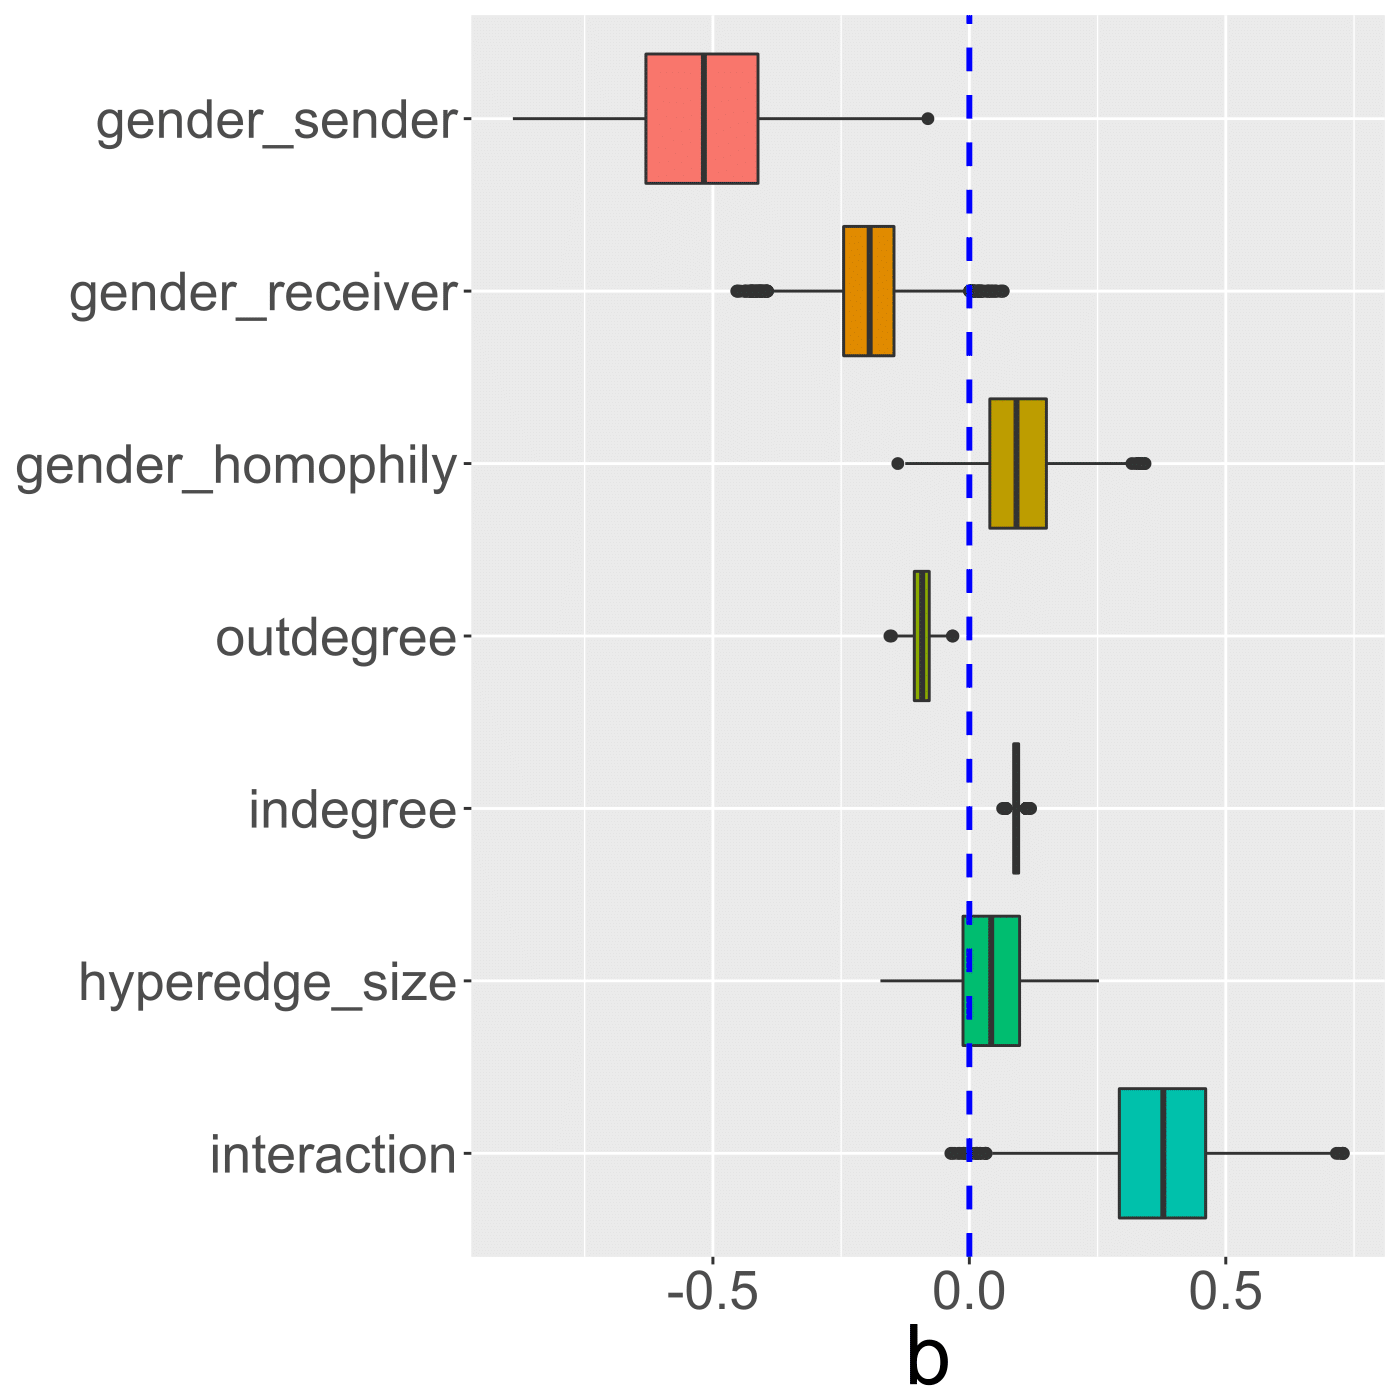
\includegraphics[width=\textwidth]{img/betanewplot2-1.png}	
					\end{subfigure}
					\begin{subfigure}[b]{0.4975\textwidth}
						\caption{Dyadic and triadic covariates}
						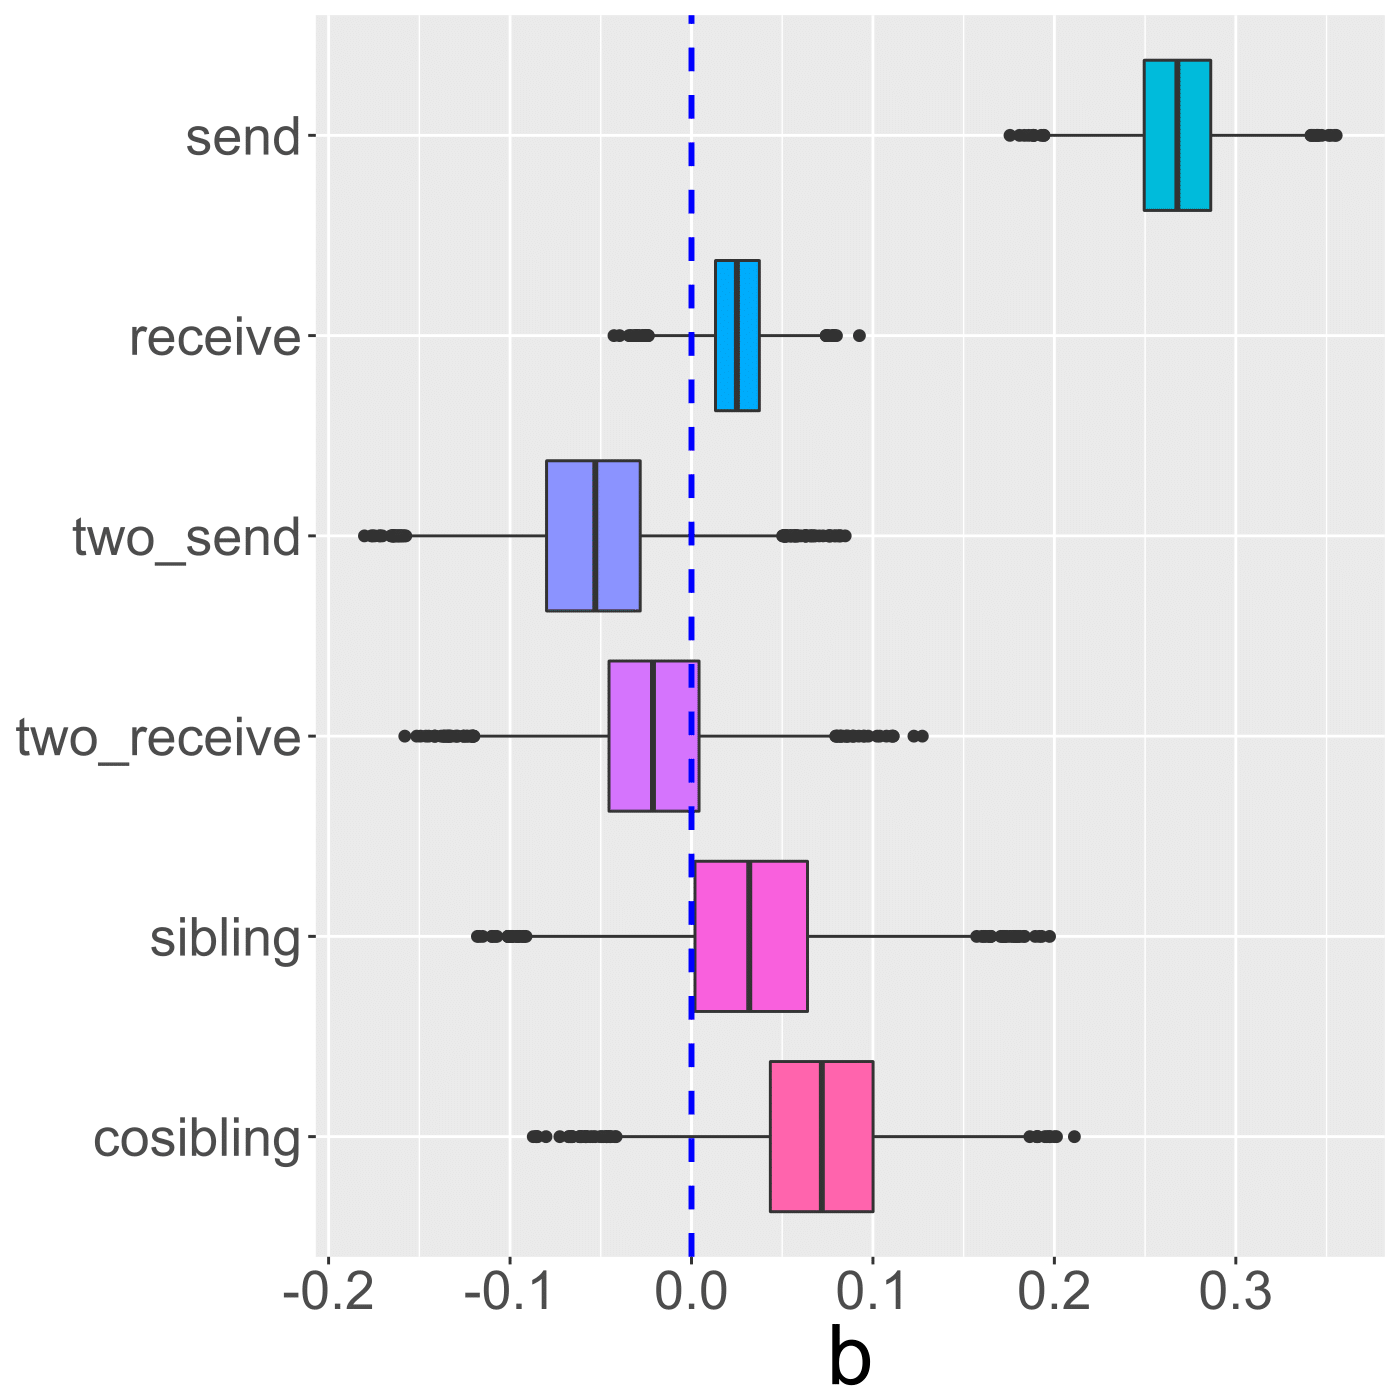
\includegraphics[width=\textwidth]{img/betanewplot3-1.png}	
					\end{subfigure}
				\end{tabular}
				\caption {Posterior distribution of $\boldsymbol{b}$ estimates.}
				\label{figure:betaresults}
			\end{figure}
	\subsubsection{Coefficients for timestamp covariates}
	For timestamp covariates, Figure \ref{figure:etaresults} shows the boxplots summarizing posterior samples of $\boldsymbol{\eta}$. Note that interpretations of the estimated coefficients for $\hat{\boldsymbol{\eta}}$ should be based on the specified timeunit of the datset, which we use ``hour" for Montgomery county email data. Moreover, since we assume log-normal distribution for time increments, the coefficients are interpreted in terms of the change in the average log time.
	\begin{equation*}
		\begin{aligned}
			&\log(\tau_{ad}) \sim N(\mu_{ad}, \sigma_\tau^2), \mbox{ with }\\
			&\mu_{ad} = \eta_{1}+\eta_{2} y_{ad2}\ldots+\eta_{7}y_{ad7}.
		\end{aligned}
	\end{equation*}
	The posterior estimates of two temporal effects---``weekend" and ``PM"---indicate that if the ${(d-1)}^{th}$ email was sent during the weekend or after midday, then the time to $d^{th}$ email is expected to take $\exp(1.552)\approx 4.722$ hours and $\exp(0.980)\approx2.665$ hours longer, respectively, compared to their counterparts (i.e., weekdays and am). On the contrary, the covariates ``manager", ``outdegree", and ``indegree"  shorten the amount of time to next email. For example, being a county manager (i.e., the lead county administrator) lowers the expected value of $\log(\tau_{ad})$ by $\hat{\eta}_3 = -1.070$, since the manager in general sends or receives a lot more emails which may shorten the response time and many of those emails. The posterior estimates for the  ``outdegree" and ``indegree" statistics, where the posterior means are approximately $\hat{\eta}_4=-0.206$ and $\hat{\eta}_5=-0.060$, respectively. These effects indicate that those who are involved in either sending or receiving a lot of emails recently are likely to send emails with greater speed. The posterior distribution for the effect of the gender of the manager is pretty evenly spread around zero. In addition, the posterior mean estimates for variance parameter $\sigma^2_\tau$ in the lognormal distribution is approximately $\hat{\sigma}^2_\tau=14.093$ with its 95\% credible interval $(12.709, 15.555)$, indicating that there exists large variability in the time increments of emails.
			\begin{figure}[!t]
				\centering
				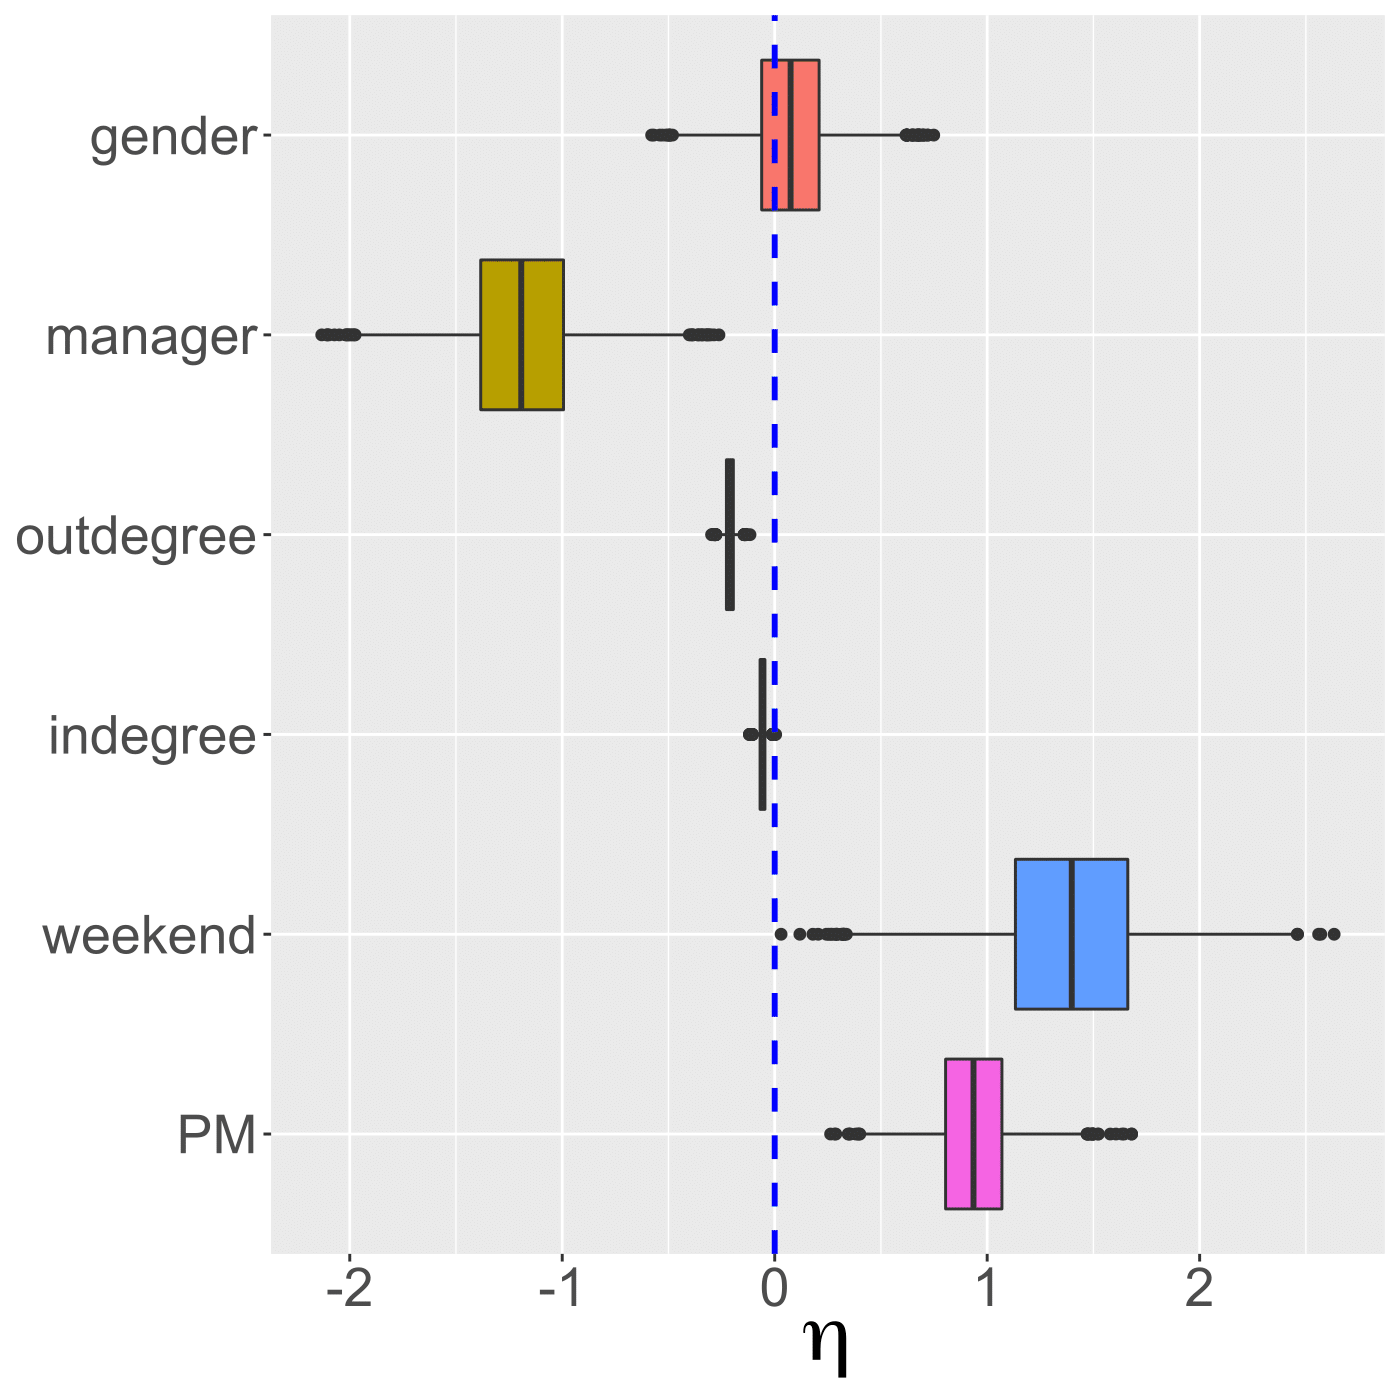
\includegraphics[width=0.4975\textwidth]{img/etaplotnew-1.png}	
				\caption {Posterior distribution of $\boldsymbol{\eta}$ estimates.}
				\label{figure:etaresults}
			\end{figure}	
	\section{Conclusion}\label{sec:conclusion}
	Motivated by a growing class of dynamic network models which deal with edges exchanged in continuous time, the hyperedge event model (HEM) can effectively learn the underlying dynamics in edge and timestamp formations, providing novel insights to the literature. The HEM explicitly models hyperedges through a receiver-selection distribution that forces the sender to select at least one recevier, which is a more realistic approach for events with one sender and one or more receivers and one or more sender and one receiver compared to treating them as pure duplicates. In modeling the timestamps (more precisely time increments) of events, our generalized linear model (GLM) based formulation offers new innovations by eliminating the need to stick with one parameter distribution (e.g., exponential distribution). To our knowledge, the HEM is the only existing model that can be used to generate the sender, recipients, and time stamp of interactions in real time. To make better use of the proposed model, we provide an algorithm for predictive experiments that help to learn which specification of HEM provides a better fit to the data. 
	
	We have demonstrated the effectiveness of our model by analyzing Montgomery County government emails, where emails serve as a canonical example of directed edges with one sender and one or more receivers. The estimated effects for edge covariates reveal that the HEM is able to understand the structural dynamics similar to those used in the exponential random graph model (ERGM), but we also learn about the effects of timestamp covariates by integrating a survival model for event timing. Although we illustrate the entire framework and application in the context of one type of hyperedge, one sender and one or more receivers, our model can be easily extended to allow the opposite case, one or more sender and one receiver, by slight modification of the generative process (shown in Appendix A). This extension involves promising applications to socio-political networks such as international sanctions and co-sponsorship of bills, and biological networks such as those formed through neural dendrites. %Furthermore, while the model's applicability is limited to small-sized networks since we assume fixed set of nodes across entire timepoints, we can adjust the model to allow time-varying nodes or improve its computational efficiency such that the model is well applicable to large-scale networks. Considering the recent explosion of network dataset with huge number of nodes (e.g., online comnunications), the development of model adjustments for better applicability are the object of future work.
	\begin{acknowledgement}
		This work was supported in part by the University of Massachusetts Amherst Center for Intelligent Information Retrieval and in part by National Science Foundation grants DGE-1144860, SES-1619644, and CISE-1320219. Any opinions, findings, and conclusions or recommendations are those of the authors and do not necessarily reflect those of the
		sponsors.
	\end{acknowledgement}
	
	\section*{Appendix}
	\subsection*{Appendix A: Alternative generative process} \label{appendix:alternativeGP}
	\begin{algorithm}[H]
		\SetAlgoLined
		\caption{Generative Process: one receiver and one or more senders}
		\begin{algorithmic}
			\STATE \textbf{Input}: number of edges and nodes $(D, A)$, covariates $(\boldsymbol{x}, \boldsymbol{y})$, and the coefficients $(\boldsymbol{b}, \boldsymbol{\eta})$
			\vskip 0.1in				
			\FOR{d=1 to D}
			\FOR{r=1 to $A$}
			\FOR{a=1 to $A$ (a $\neq$ r)}
			\STATE	set $\lambda_{adr} = {\boldsymbol{b}}^{\top}\boldsymbol{x}_{adr}$
			\ENDFOR
			\STATE	draw $\boldsymbol{u}_{rd}  \sim
			\mbox{MB}_G(\boldsymbol{\lambda}_{rd})$
			\STATE		set $\mu_{rd} = g^{-1}(\boldsymbol{\eta}^\top \boldsymbol{y}_{rd})$
			\STATE		draw $\tau_{rd} \sim f_\tau(\mu_{rd}, \sigma_\tau^2)$
			\ENDFOR
			\IF {$n \geq 2$ tied events} 
			\STATE	set ${r}_d=\mbox{argmin}_{r}(\tau_{rd})$
			\STATE	set $\boldsymbol{a}_d=\boldsymbol{u}_{r_d d},\ldots,\boldsymbol{a}_{d+n-1}=\boldsymbol{u}_{r_{d+n-1} d}$
			\STATE	set $t_d, \ldots, t_{d+n-1}=t_{d-1} + \min_r\tau_{rd}$
			\STATE		jump to $d = d+n$
			\ELSE
			\STATE	set ${r}_d = \mbox{argmin}_{r}(\tau_{rd}) $
			\STATE	set $\boldsymbol{a}_d= \boldsymbol{u}_{r_d d}$
			\STATE	set $t_d =t_{d-1} + \min_r\tau_{rd}$
			\ENDIF
			\ENDFOR
		\end{algorithmic}
		\label{alg:generative2}
	\end{algorithm}
		\subsection*{Appendix C: Comparison of PPC results: log-normal vs. exponential}\label{appendix: PPCexp}
		\begin{figure}[H]
			\centering
			\begin{tabular}[t]{cc}
				\begin{subfigure}[b]{0.495\textwidth}
					\caption{Outdegree distribution}
					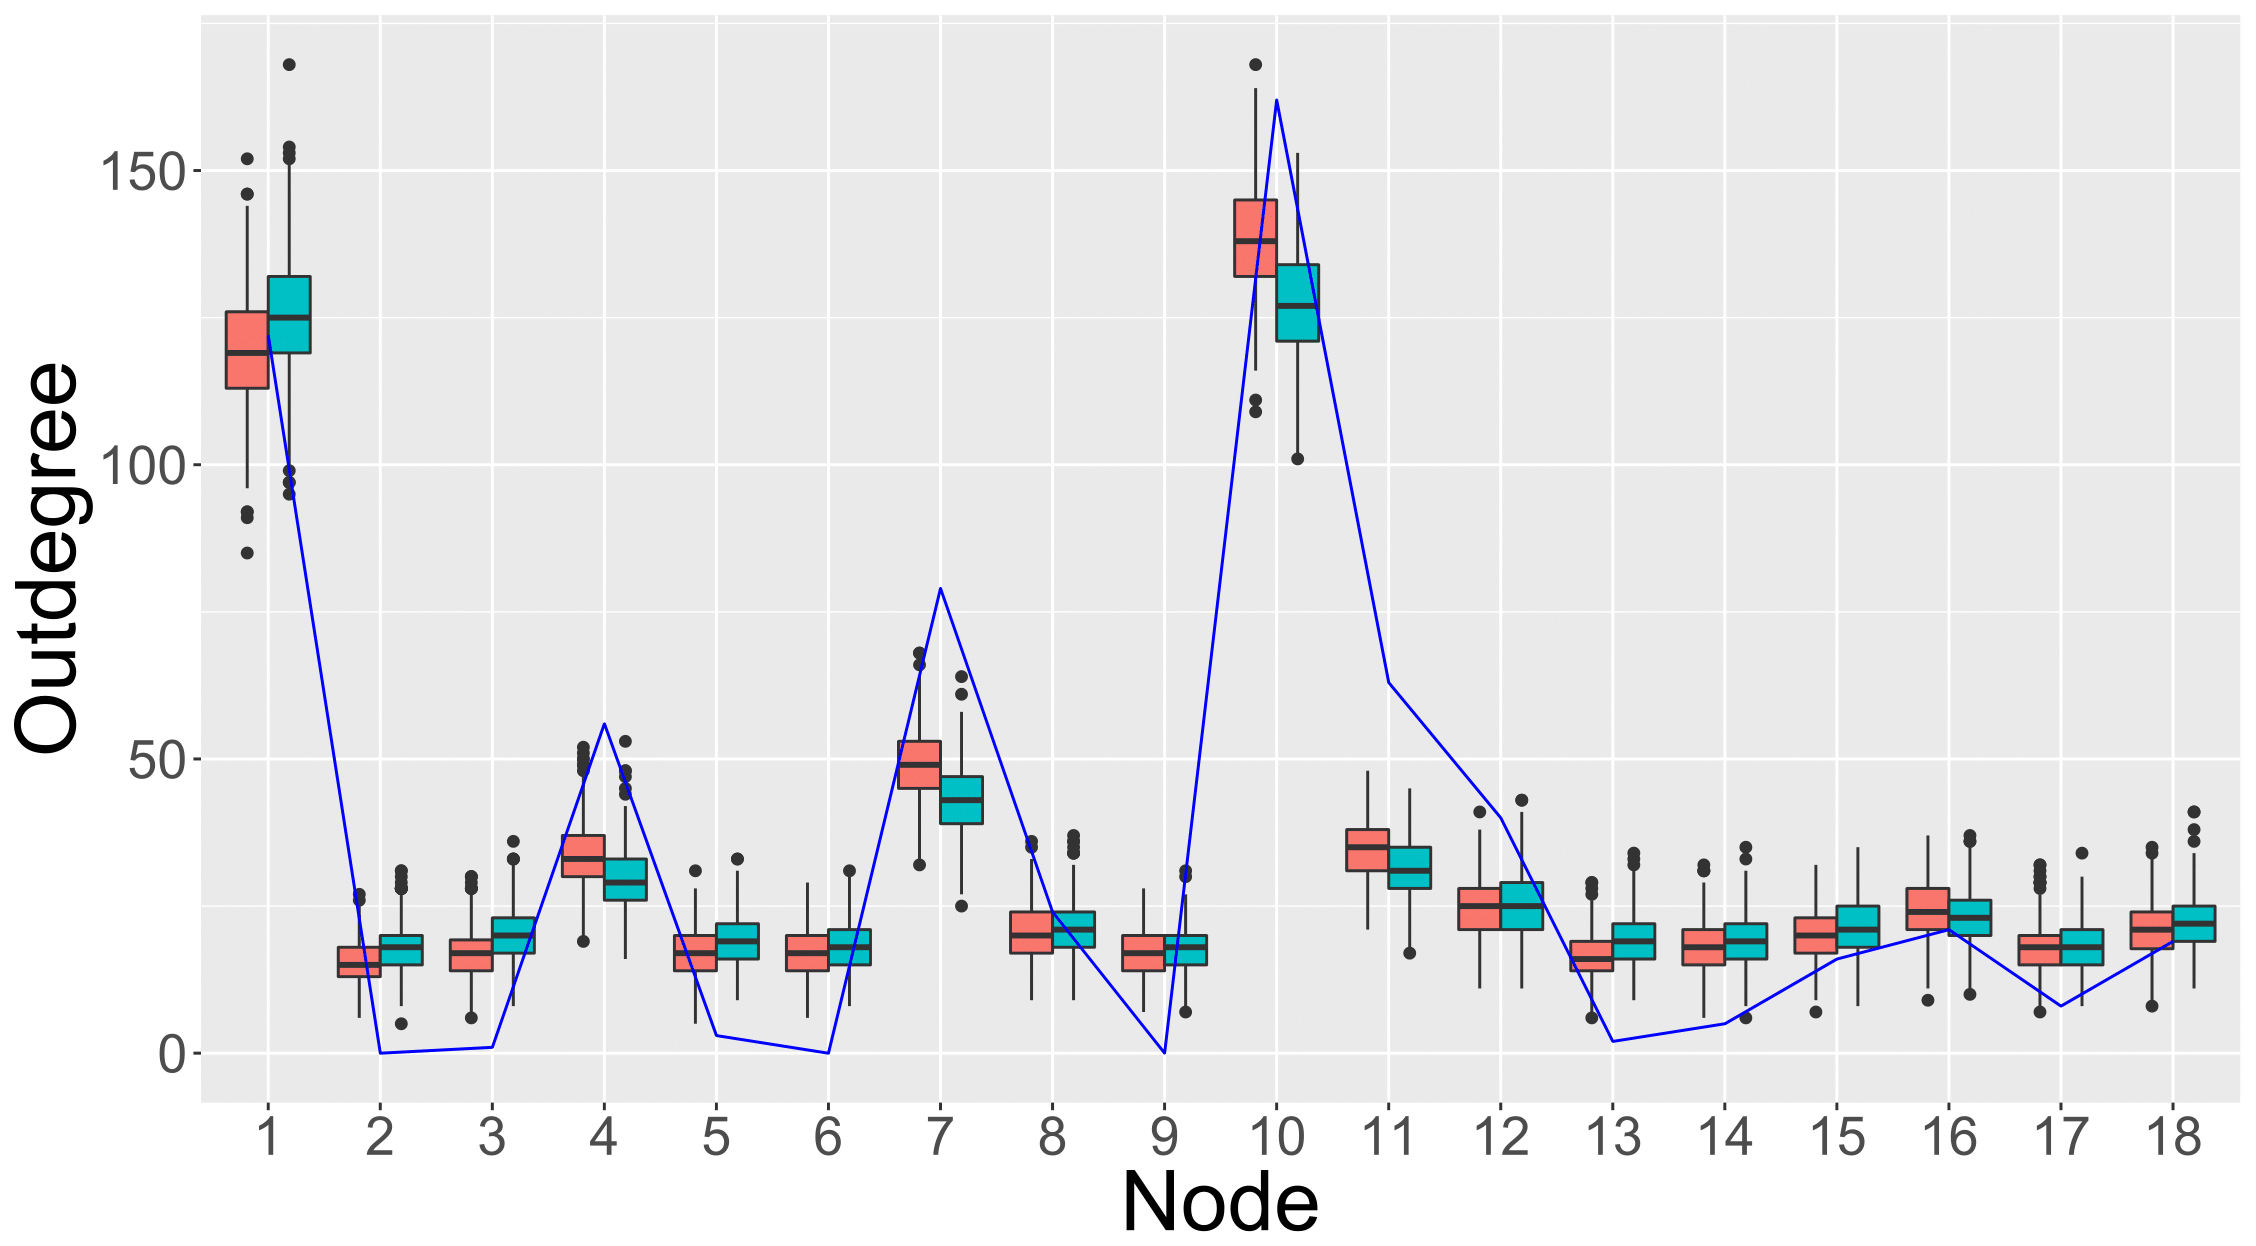
\includegraphics[width=\textwidth]{img/outdegree2-1.png}	
				\end{subfigure}
				\begin{subfigure}[b]{0.495\textwidth}
					\caption{Indegree distribution}
					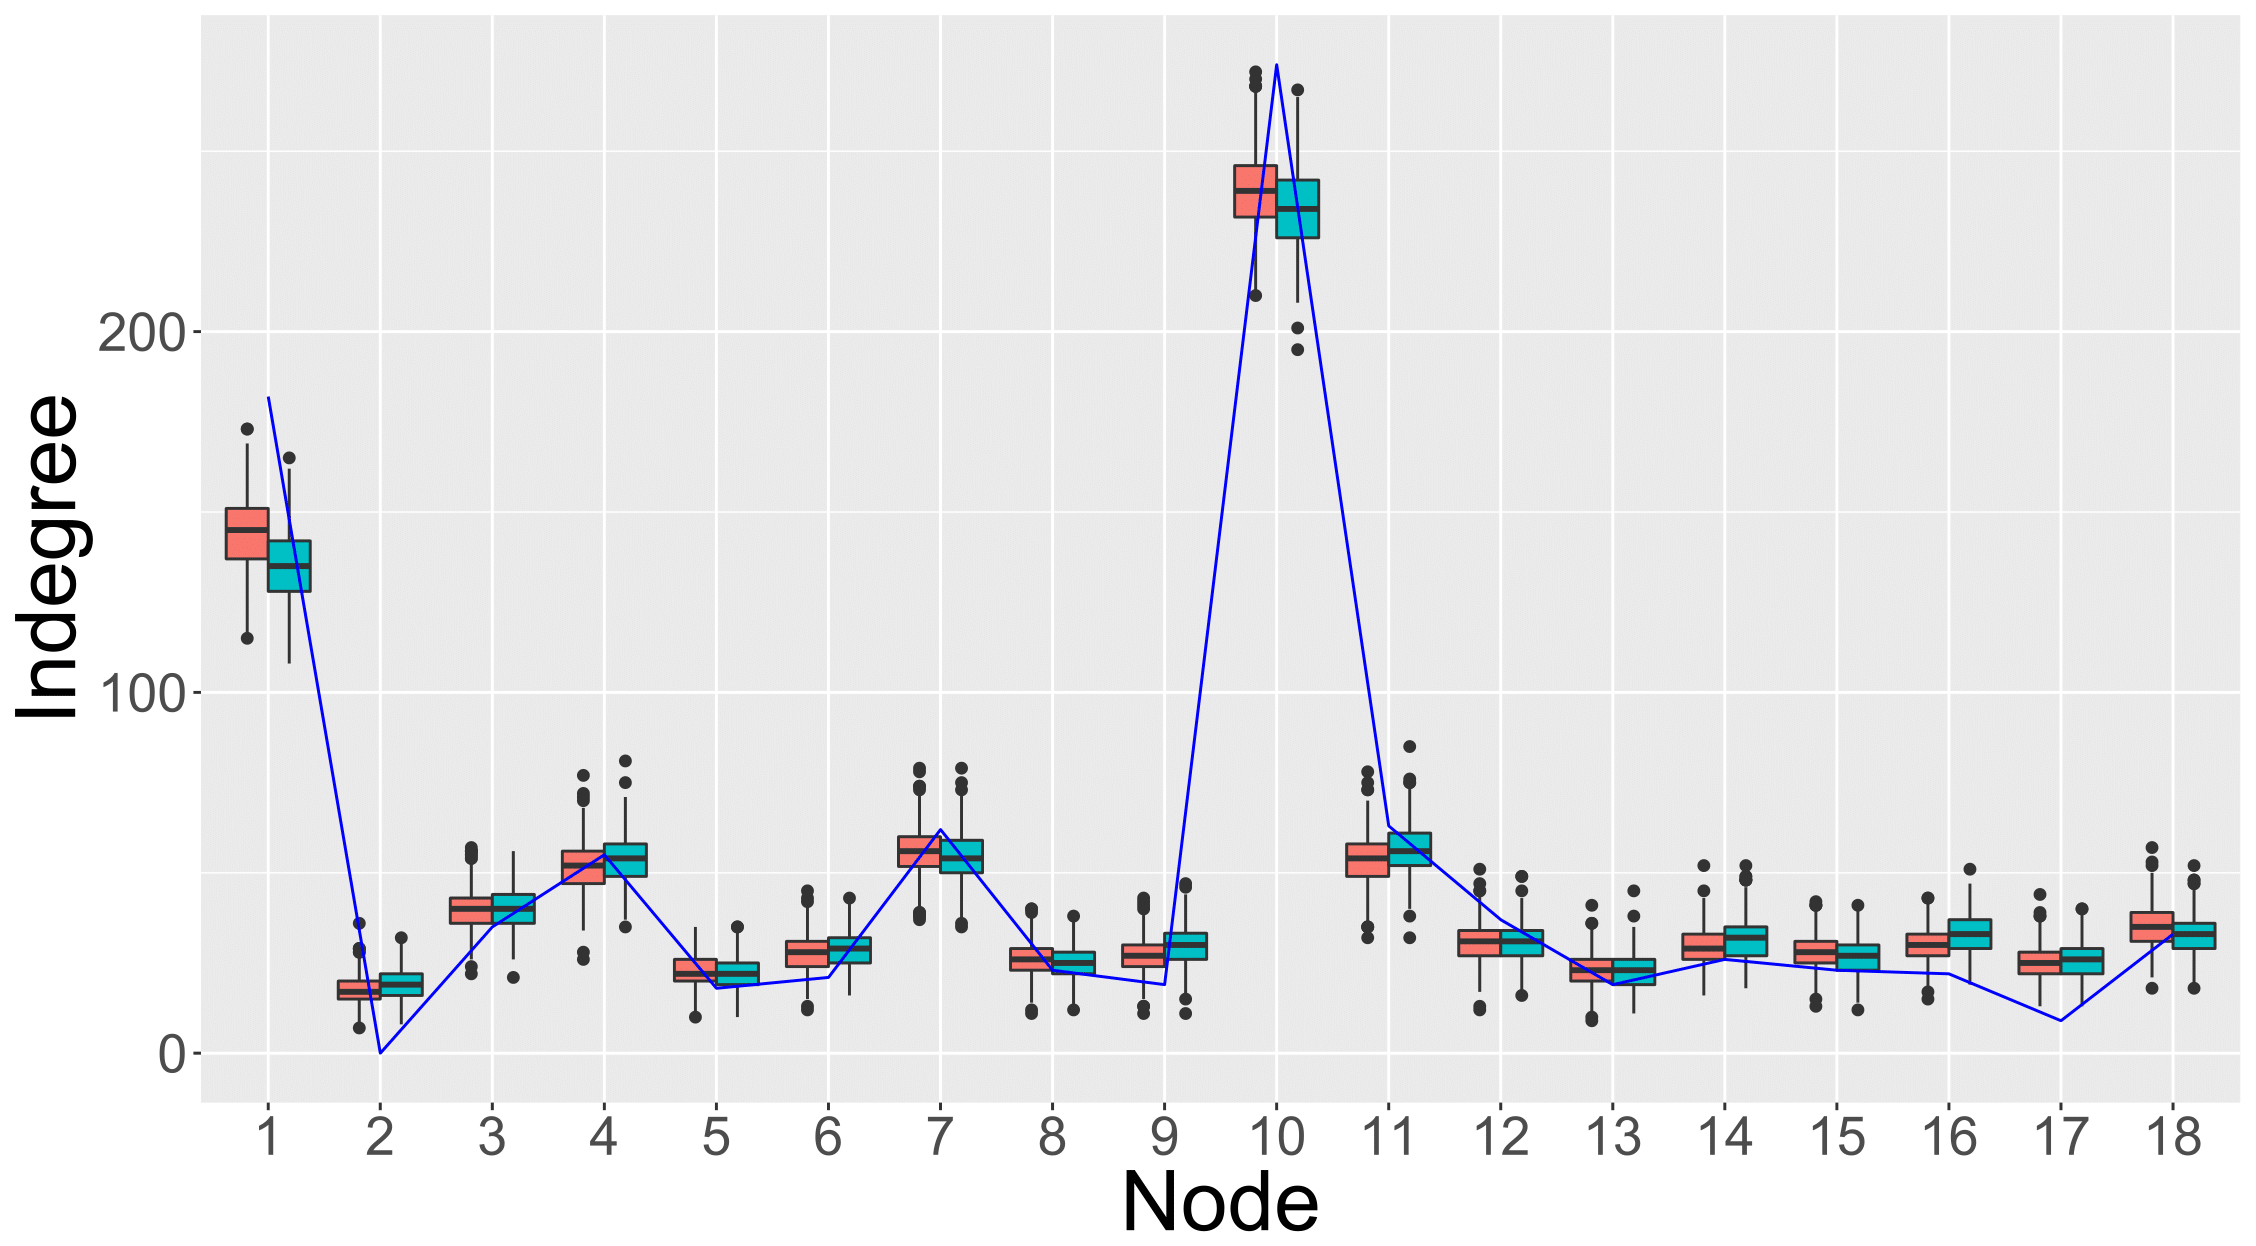
\includegraphics[width=\textwidth]{img/indegree2-1.png}	
				\end{subfigure}\\
				\begin{subfigure}[b]{0.495\textwidth}
					\caption{Receiver size distribution}
					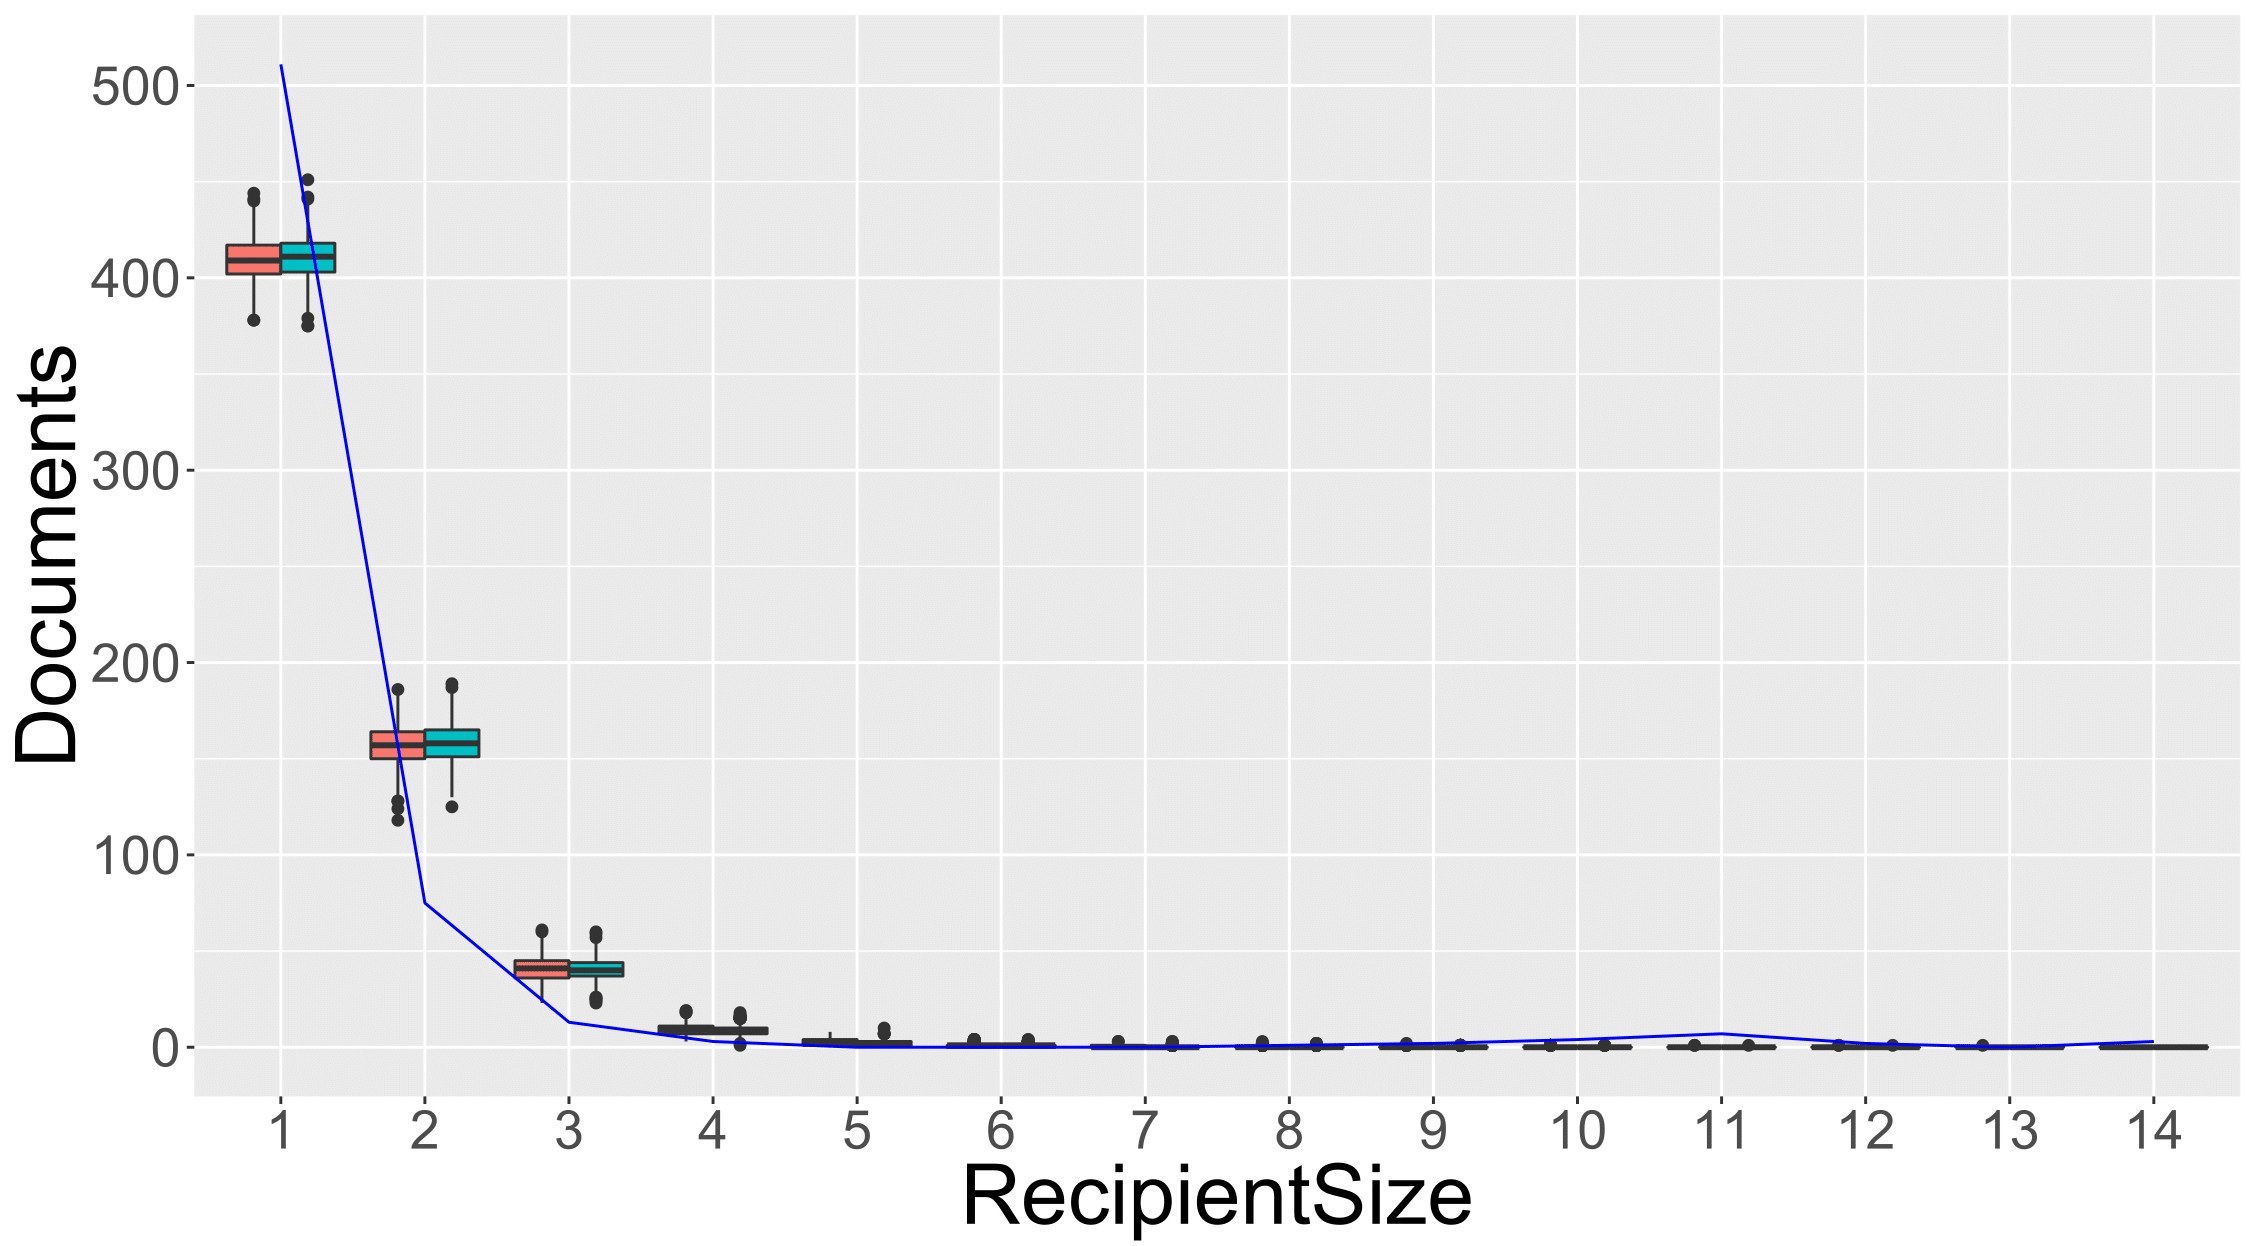
\includegraphics[width=\textwidth]{img/recipientsize2-1.png}	
				\end{subfigure}
				\begin{subfigure}[b]{0.495\textwidth}
					\centering
					\caption{PPplot for time increments}
					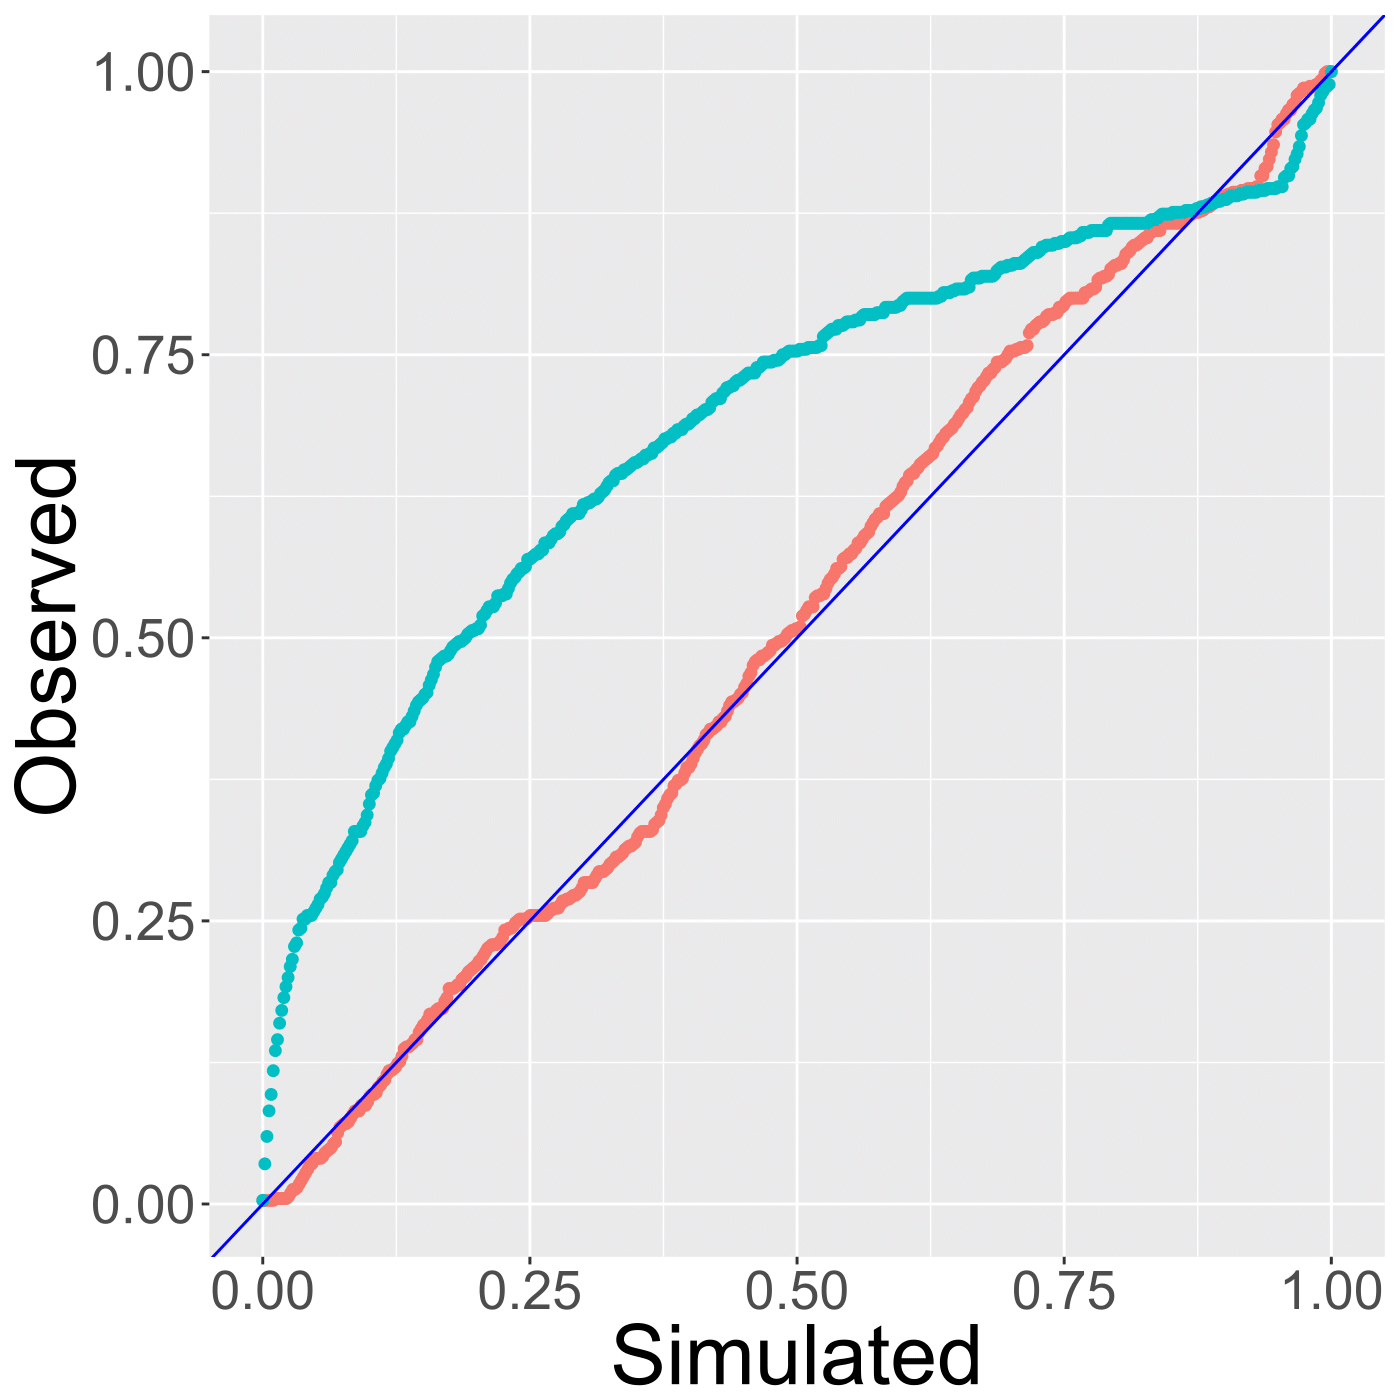
\includegraphics[width=0.56\textwidth]{img/timePPplot2-1.png}
				\end{subfigure}
			\end{tabular}
			
\includegraphics[width=0.4\textwidth]{img/modellabel.png}
			\caption {Comparison of PPC results between log-normal (\textit{red}) and exponential (\textit{green}) distributions. Blue lines denote the observed statistics in (a)--(c) and denotes the diagonal line in (d).}
			\label{figure:PPCtwo}
		\end{figure}
		\newpage
		\subsection*{Appendix D: Convergence diagnostics}\label{appendix: convergence}
		\begin{figure}[H]
			\centering
			\begin{tabular}[t]{cc}
				\begin{subfigure}[b]{0.495\textwidth}
					\caption{Traceplots of $\boldsymbol{b}$}
					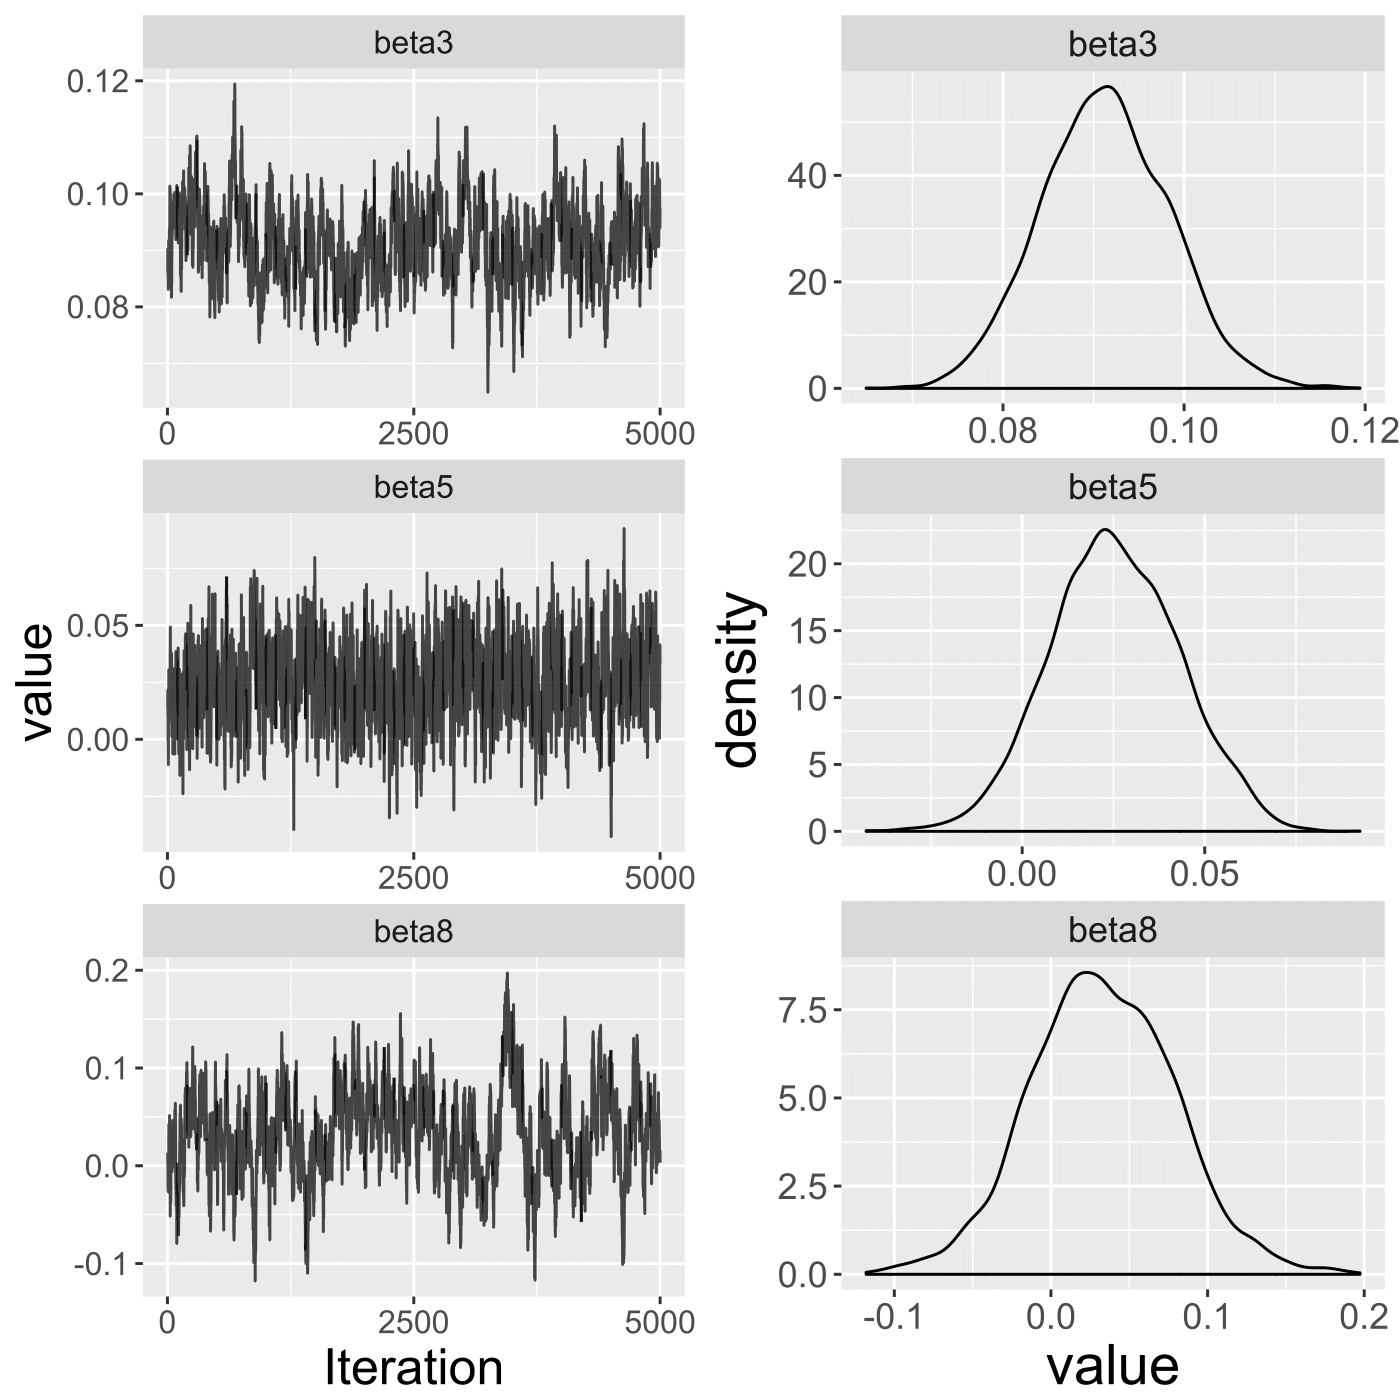
\includegraphics[width=\textwidth]{img/betatrace-1.png}	
				\end{subfigure}
				\begin{subfigure}[b]{0.495\textwidth}
					\caption{Traceplot of $\boldsymbol{\eta}$}
					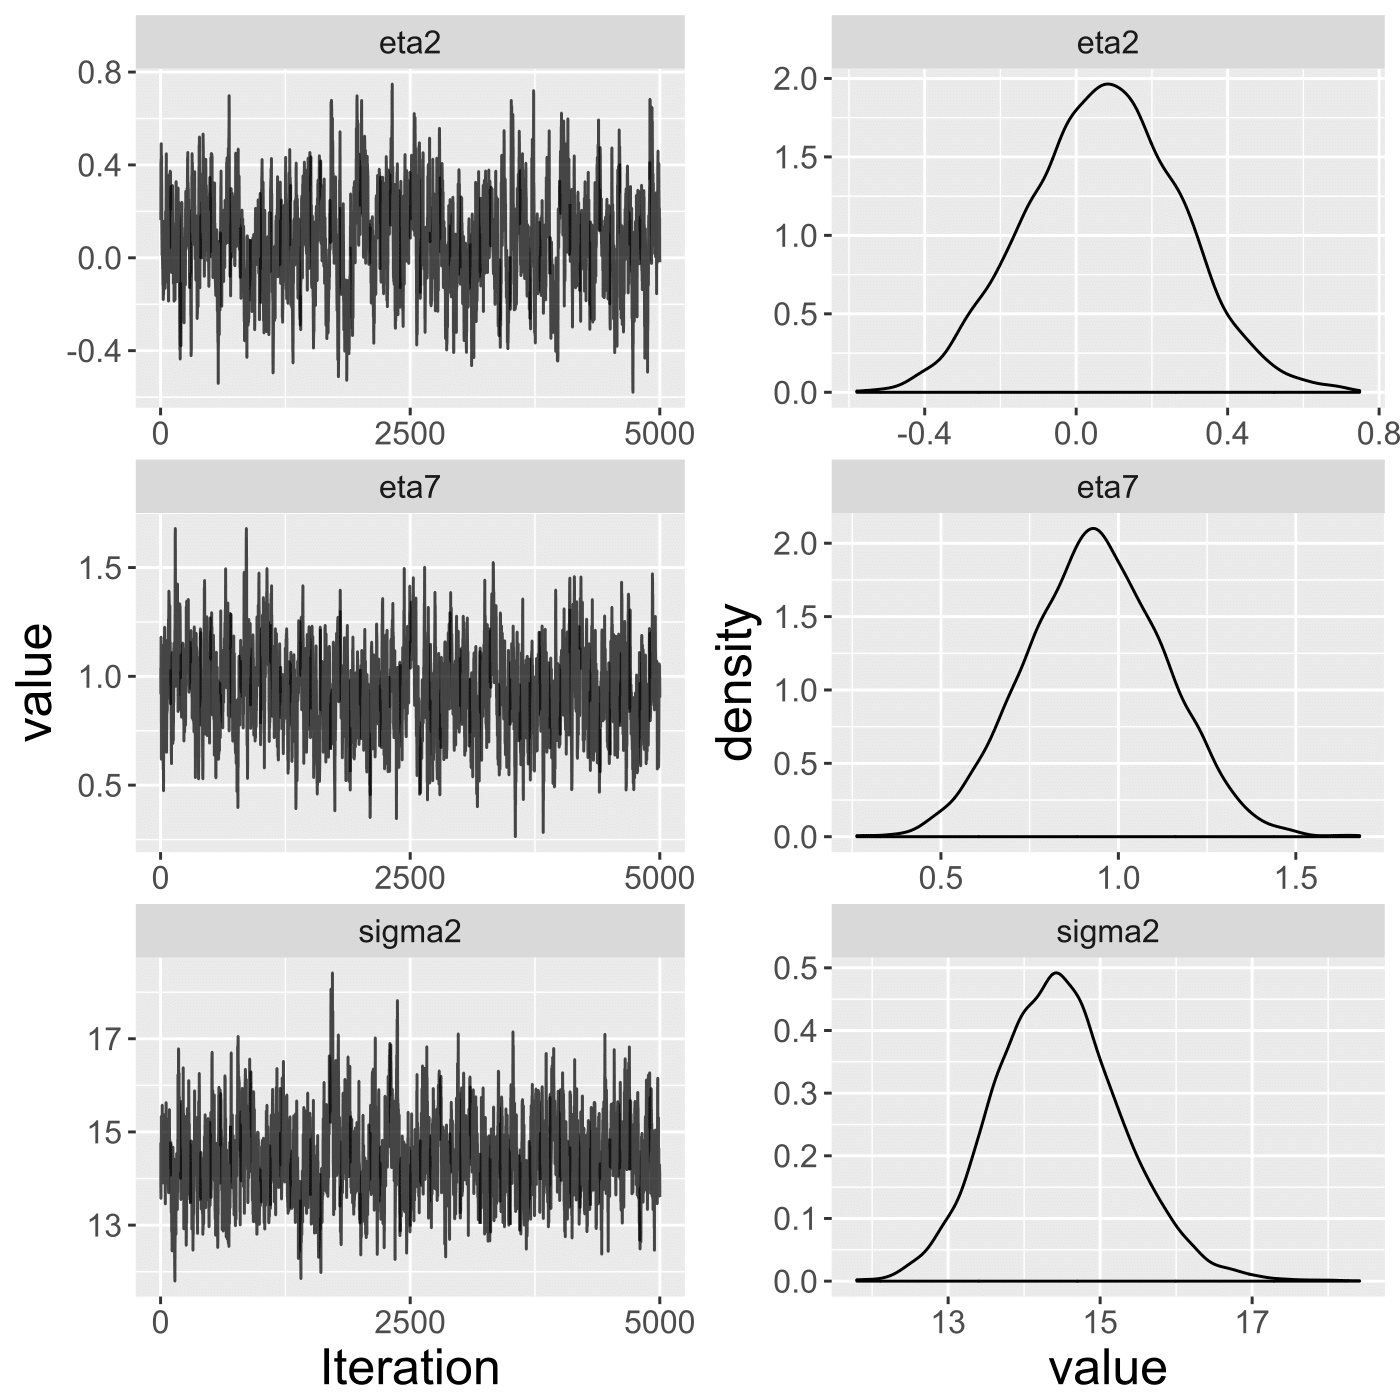
\includegraphics[width=\textwidth]{img/etatrace-1.png}	
				\end{subfigure}\\
				\begin{subfigure}[b]{0.495\textwidth}
					\caption{Geweke diagnostics for $\boldsymbol{b}$}
					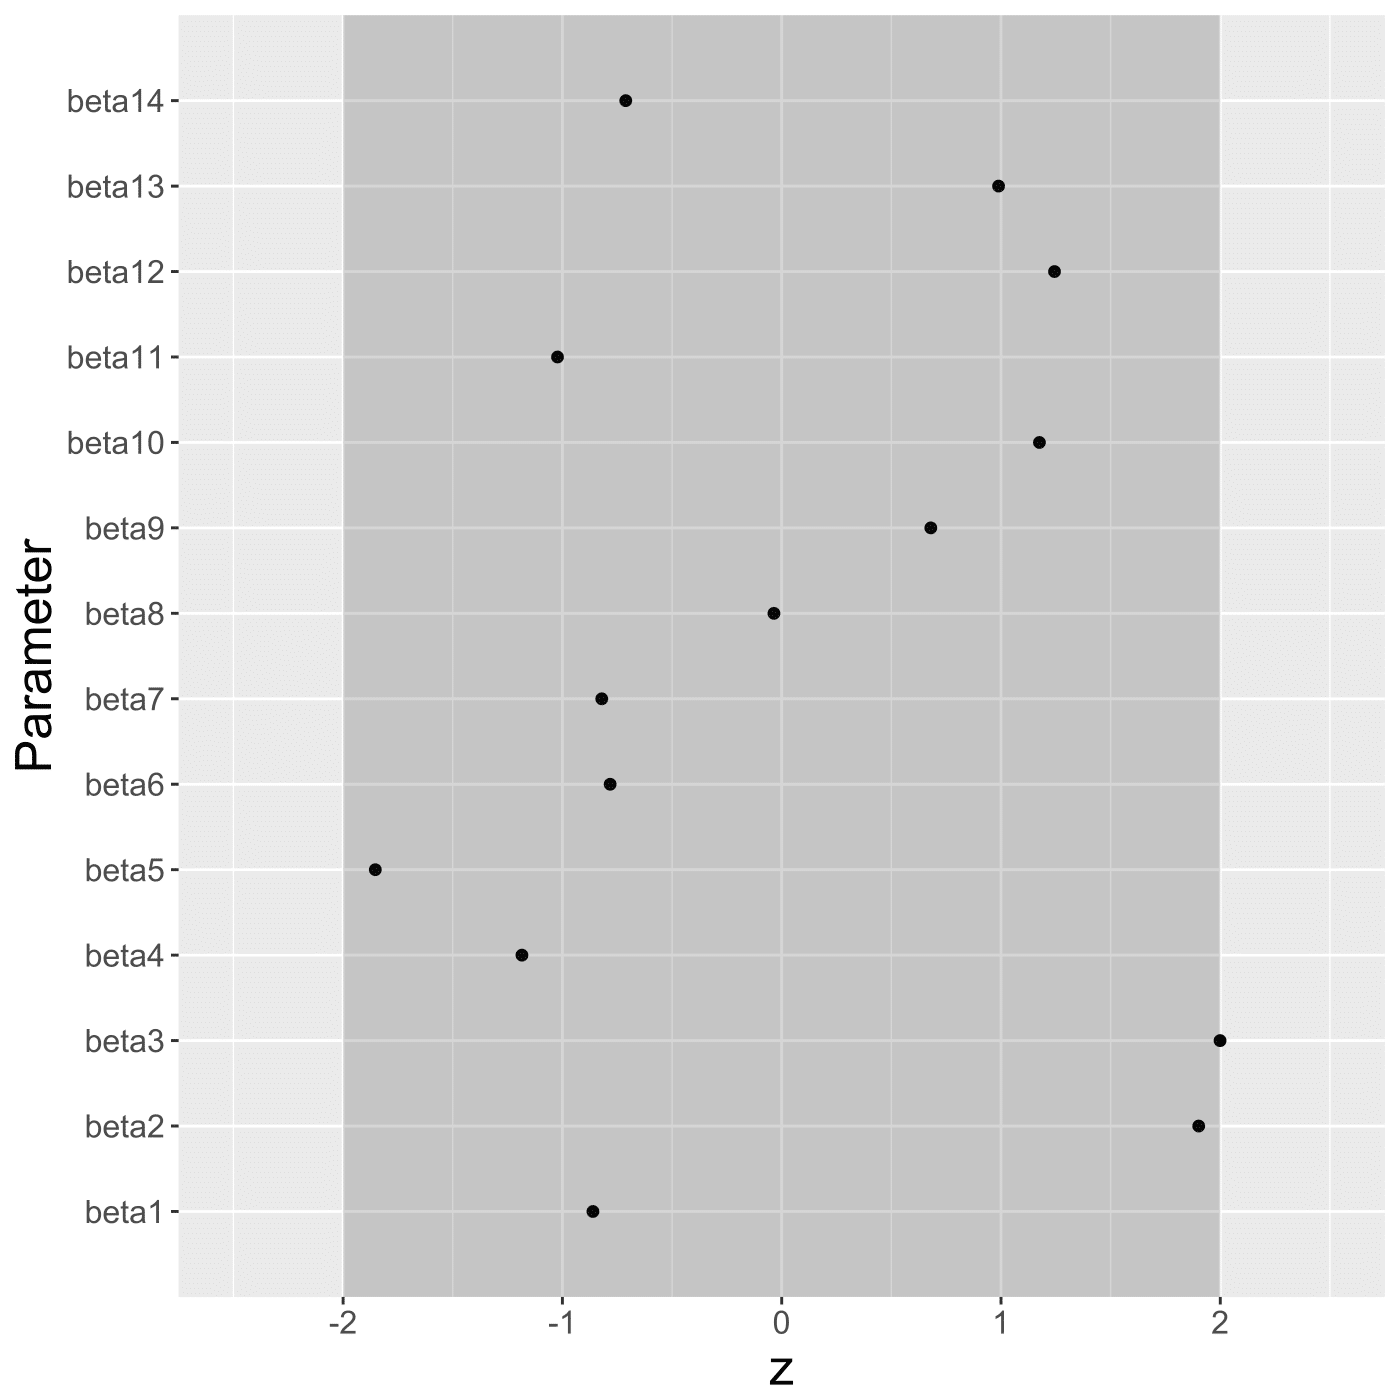
\includegraphics[width=\textwidth]{img/betageweke-1.png}	
				\end{subfigure}
				\begin{subfigure}[b]{0.495\textwidth}
					\centering
					\caption{Geweke diagnostics for $\boldsymbol{\eta}$ and $\sigma^2_\tau$}
					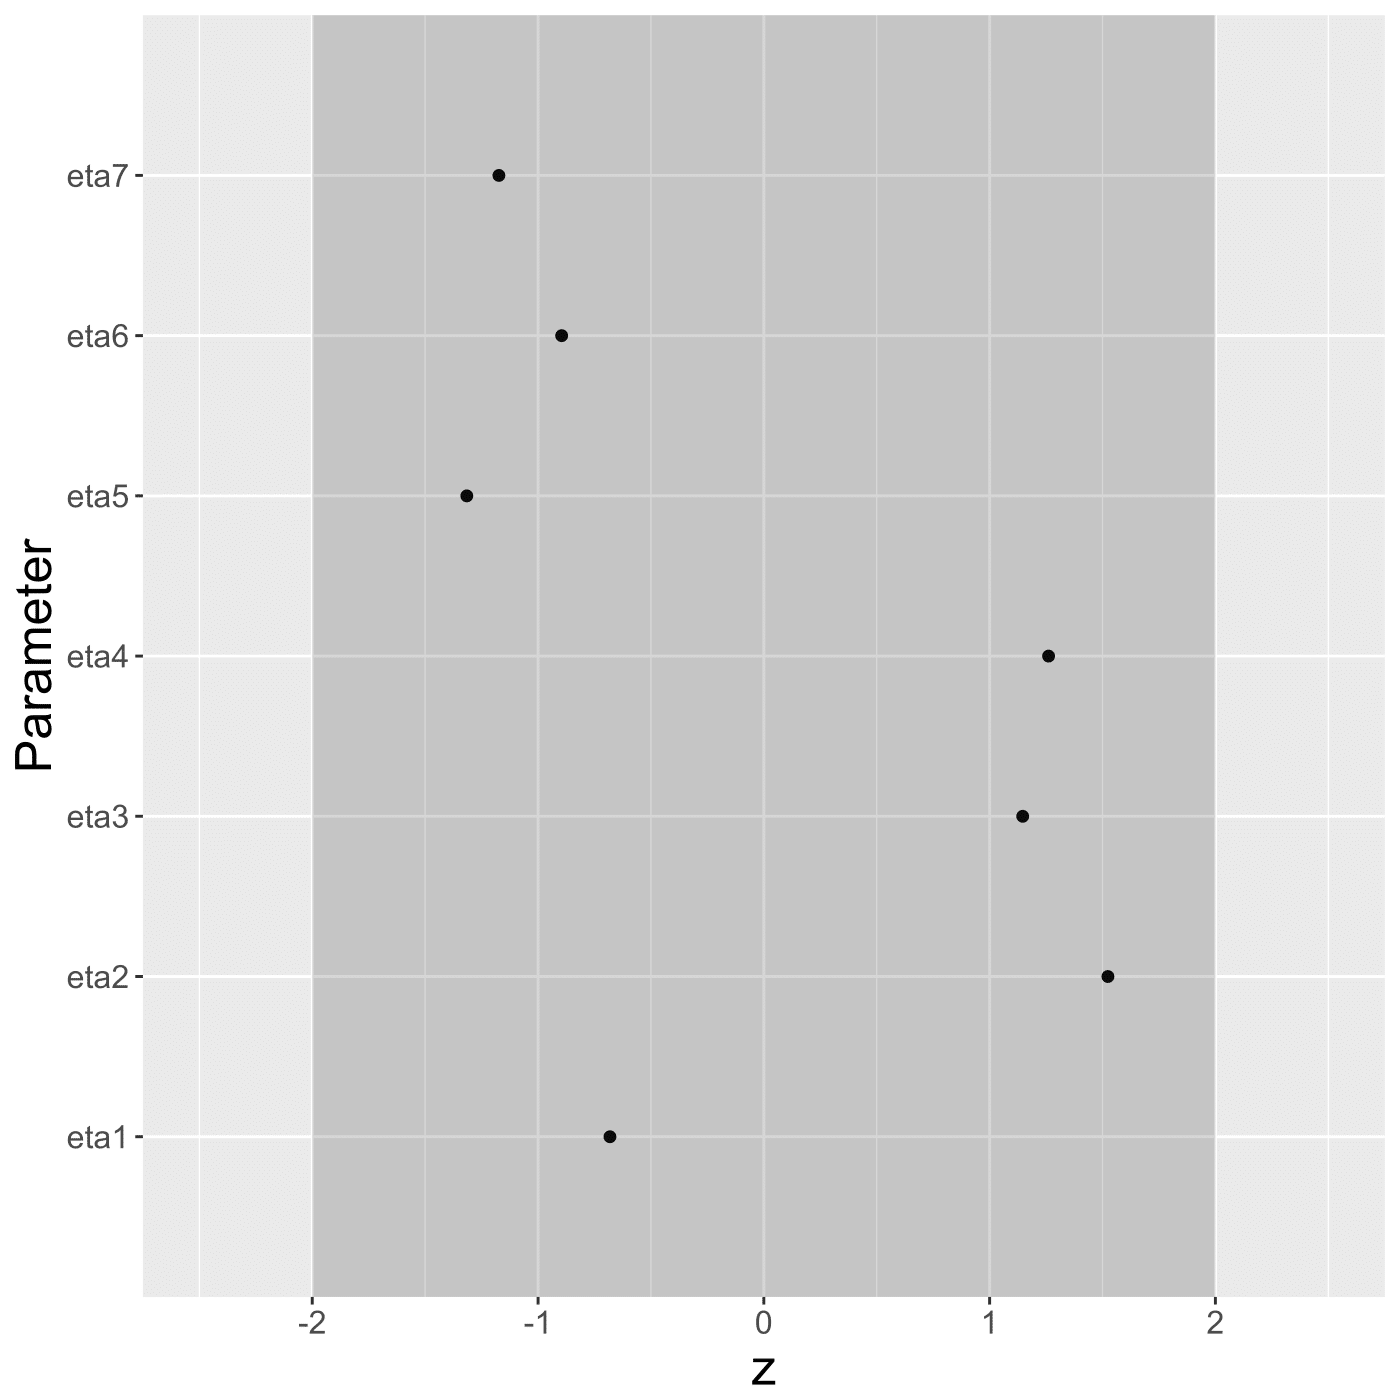
\includegraphics[width=\textwidth]{img/etageweke-1.png}
				\end{subfigure}
			\end{tabular}
			\caption {Convergence diagnostics from log-normal distribution.}
			\label{figure:convergencediag}
		\end{figure}
		
		\iffalse
		\begin{supplement}
			\sname{Supplement A}\label{suppA} 
			\stitle{Title of the Supplement A}
			\slink[url]{http://www.some-url-address.org/dowload/0000.zip}
			\sdescription{Add description for supplement material.}
		\end{supplement}
		\fi
			\fi
		\bibliographystyle{ba}
	\bibliography{baIPTM}
		
		
	\end{document}

